\section{Introduction}
One of the major goals of the global neutrino physics programme is to explore fundamental symmetries of nature linked to why we live in a matter-dominated universe. 
Charge-parity symmetry violation (CPV) in the neutrino sector is one possibility remaining to be explored further experimentally, and neutrino experiments strive to improve current measurements of CPV in the leptonic sector~\cite{Abe:2019vii}. 
CPV is obtained from the simultaneous fit of the $\nu_{\mu}$ disappearance and $\nu_e$ appearance oscillation channels separately for neutrinos and anti-neutrinos.
In the absence of CPV and accounting for matter effects, the rates of $\nu_{\mu}\!\rightarrow\!\nu_e$ and $\overline{\nu}_{\mu}\!\rightarrow\!\overline{\nu}_e$ oscillations should be equal.
%CPV searches compare the number of $\nu_{\mu}\!\rightarrow\!\nu_e$ and $\overline{\nu}_{\mu}\!\rightarrow\!\overline{\nu}_e$ oscillations, which, in the absence of CPV and accounting for matter effects, should be equal. 
To convert the measured rate of interactions to a level of CPV, experiments must accurately know the cross section for the interactions of neutrinos and anti-neutrinos with detector materials, which are most commonly hydrogen, carbon, oxygen, argon, and iron. 
Therefore, systematic uncertainties on neutrino-nucleus interaction cross sections are a key input to such CPV searches.  
These interaction cross sections are dependent on modeling neutrino-nucleon interactions occurring within nuclei. 

The nuclear models informed by these cross sections have substantial effects on the measured final-state particle kinematic distributions~\cite{Mosel:2016cwa}.

The long baseline neutrino experiments that are currently searching for CPV are the Tokai to Kamioka experiment~(T2K)~\cite{Abe:2019vii} and the NuMI Off-Axis $\nu_{e}$ Appearance experiment~(NOvA)~\cite{Acero:2019ksn}.
The T2K experiment, which currently reports the strongest constraint on CPV in neutrinos~\cite{Abe:2019vii}, has systematic uncertainties of 7-9\% after near-detector constraint on the prediction of the rate of far detector electron-like events, with cross section uncertainties being the largest contribution.
The future Deep Underground Neutrino Experiment~(DUNE)~\cite{abi2020deep} and Hyper-Kamiokande~\cite{abe2011letter} projects will seek to reach 1-3\% on that same rate of far detector electron-like events~\cite{acciarri2016long}, with improved systematic errors providing better precision on the CP violating phase.
The key to reducing these uncertainties is to precisely measure the multiplicity and momentum distribution of final-state particles. 
However, these distributions are modified by final state interactions (FSI) of the recoiling secondary particles as they traverse the target nucleus. 
The most commonly used neutrino generator Monte Carlos (GENIE~\cite{Andreopoulos:2009rq}, NEUT~\cite{Hayato:2009zz}, and NuWro~\cite{GOLAN2012499}), simulate FSI with cascade models that are tuned with external hadron-nucleus scattering measurements. The generator GiBUU~\cite{lalakulich2013neutrino} models FSI by solving the semi-classical Boltzmann-Uehling-Uhlenbeck equation.

\begin{figure}%
    \centering
    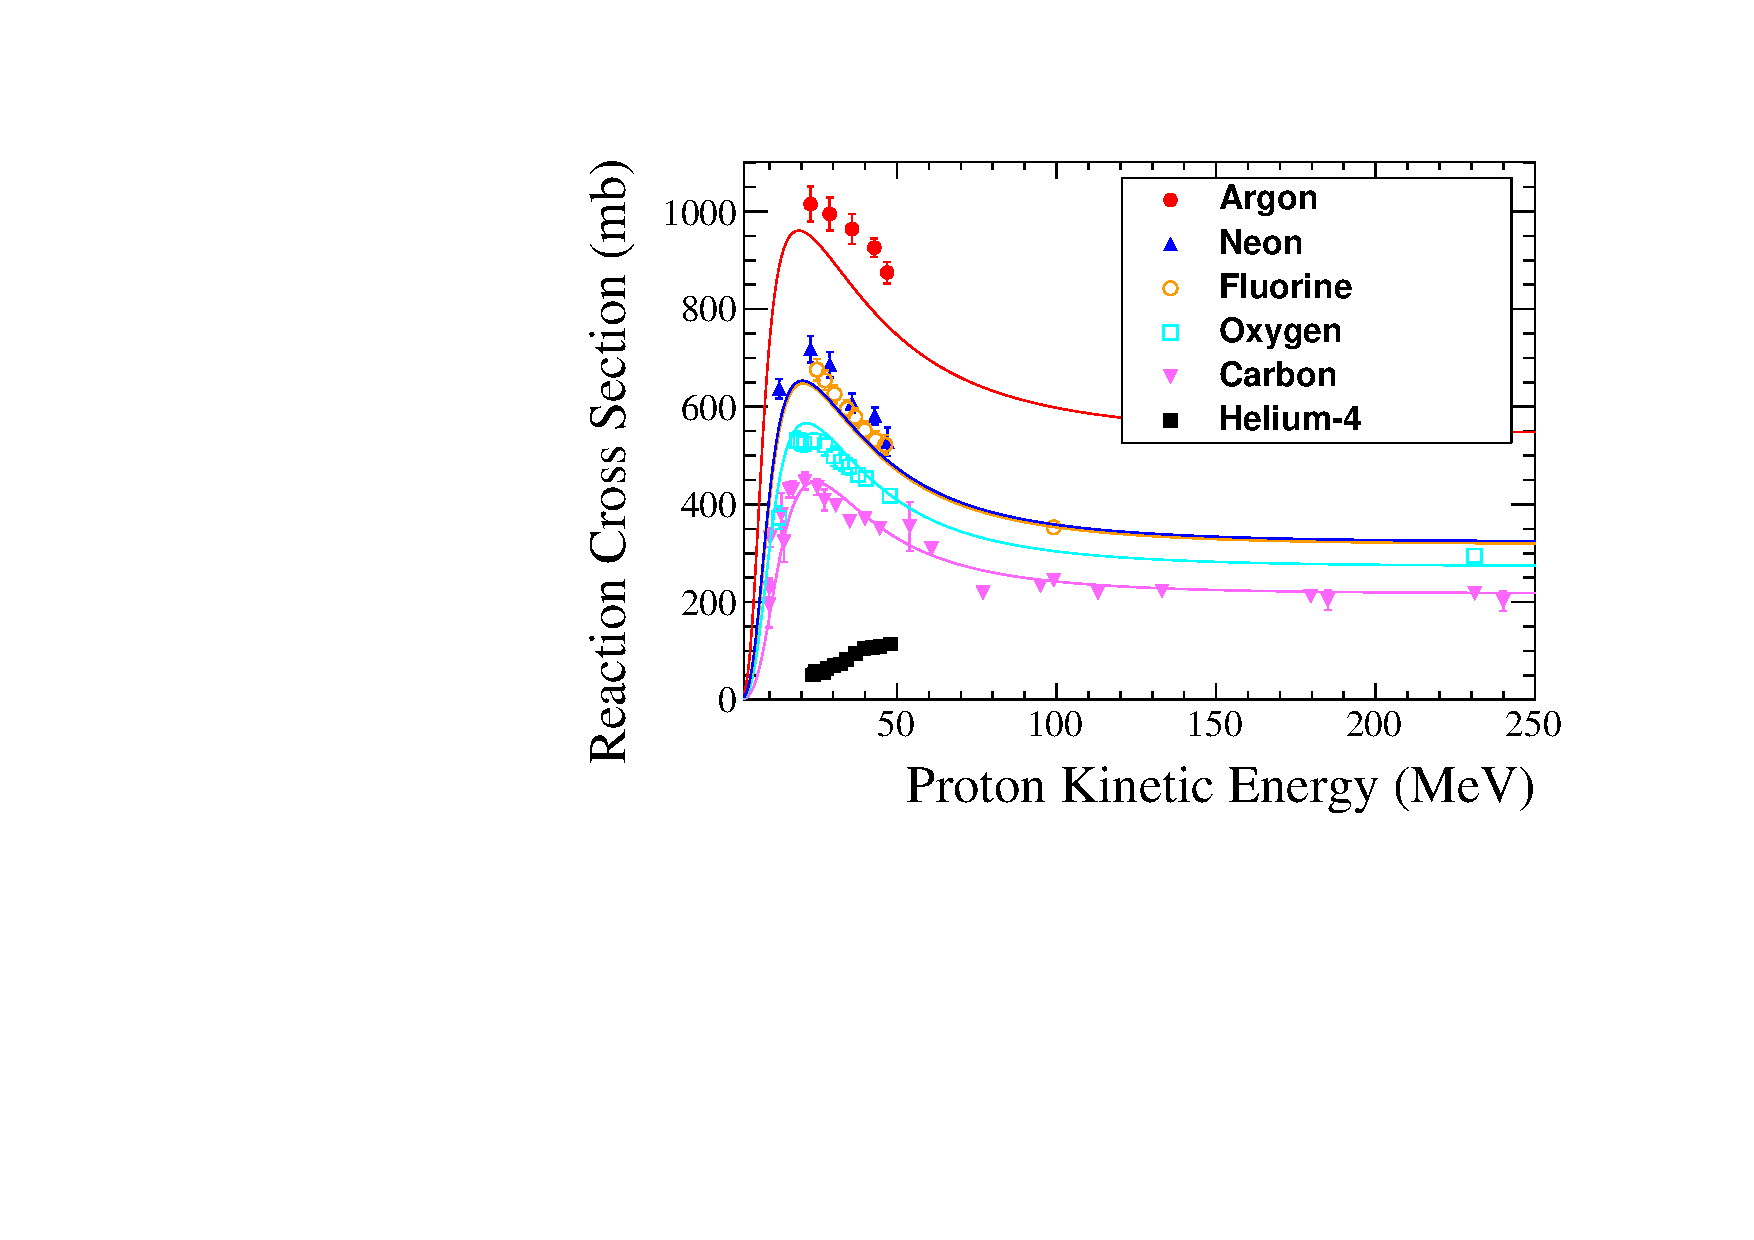
\includegraphics[width=12cm]{files/Figures/DataProtonCrossSections.pdf}%
    \caption{Total reaction cross sections for protons on argon, neon, fluorine, oxygen, carbon, and helium-4. Data~\cite{Carlson:1996ofz} are compared to a semi-empirical model~\cite{wellisch1996total}.}
    \label{fig:DataProtonXSec}%
\end{figure}

However, as shown in Figure~\ref{fig:DataProtonXSec}, proton-nucleus scattering measurements are extremely sparse and in many cases do not exist in the relevant energy region and/or on the relevant nuclei.
Therefore semi-empirical parameterisations are used to extrapolate in momentum and atomic mass~\cite{wellisch1996total}.  
The parametrisations are different between the three generators, and yield order-of-magnitude scale differences in the predicted multiplicity and kinematics of final state protons~\cite{dune2018high}.
The proton final state modeling is a key ingredient for neutrino oscillation measurements because it affects the event selection and neutrino energy reconstruction in charged-current (CC) interactions, which is the channel used to measure oscillation parameters and is therefore central to the search for CPV~\cite{Abe:2013hdq}.
For these reasons, FSI contribute substantially to the total neutrino interaction systematic uncertainty~\cite{Abe:2019vii}. 

Moreover, FSI models are in tension with data.  
Recent neutrino scattering measurements have shown that the most-used models of neutrino-nucleus interactions (employed by NEUT and GENIE) differ from nature in both cross section and kinematics of final state particles by as much as 30\%~\cite{McFarland:2018aaa}. 
These uncertainties cannot be fully mitigated with near/far detector combinations because they come from theoretical model deficiencies that are not cancelled in the near–far extrapolation~\cite{Coloma:2013rqa}. 
%To achieve 1-2\% systematic uncertainties for CPV searches, interaction models must be tuned and validated against precise proton-nucleus and pion-nucleus scattering measurements covering a broad final-state particle phase space, on a range of nuclear targets~\cite{Cao:2014zra}.

\begin{figure}%
    \centering
    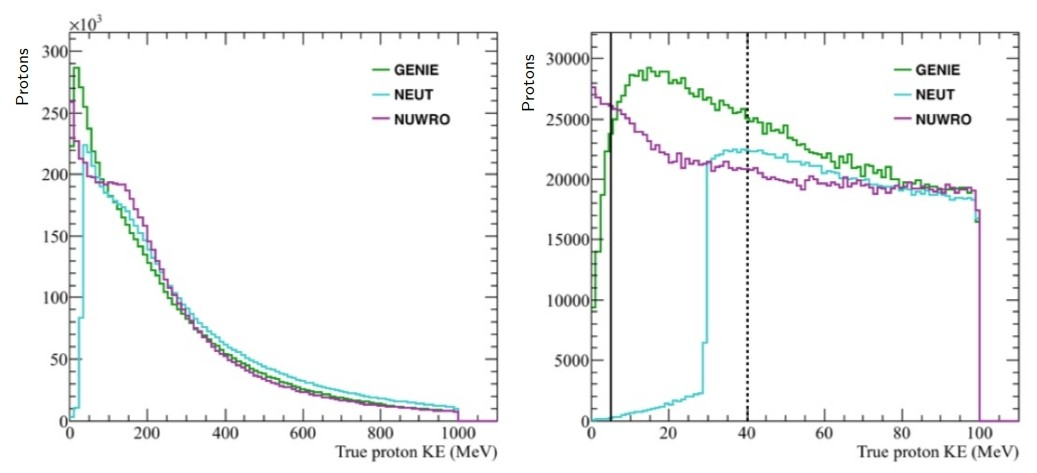
\includegraphics[width=12cm]{files/Figures/protons_from_argon.jpeg}%
    \caption{Predicted proton kinetic energy (KE) spectra from GENIE, NEUT, and NuWro\cite{Raaf:2018aaa}. Energy spectra up to 1 GeV are shown on the left, and zoomed in to lower energies on the right. The figure uses the Long Baseline Neutrino Facility (LBNF)  simulation for DUNE's beam energy and flux. The LBNF beam has a mean energy of approximately 2.5~GeV\cite{abi2020deep}. The dashed vertical line indicates the expected proton automated-reconstruction/identification threshold in liquid argon, and the solid vertical line shows the same for gaseous argon at 10 atm~\cite{dune2018high}}
    \label{fig:protonsfromargon}%
\end{figure}

The key proton kinetic energy range in which to distinguish interaction models is the region below 0.1~GeV.
Figure~\ref{fig:protonsfromargon} shows the proton multiplicity and kinetic energy distributions for $\nu_{\mu}$ CC interactions on argon calculated by the GENIE, NEUT, and NuWro neutrino generators for the DUNE experiment.
These distributions are highly discrepant at low proton kinetic energy as shown in the right hand panel. Due t
This is predominantly below the proton detection threshold in liquid Argon TPCs (0.04~GeV), such as those that will be used by DUNE, and in water Cherenkov detectors (0.5~GeV).
The lower threshold in high pressure gas provides a unique opportunity to distinguish between neutrino interaction models for the same nuclear target.

We have built a High Pressure gas Time Projection Chamber (HPTPC) prototype and exposed it to a charged particle beam in the T10 beamline at CERN in August and September 2018 \cite{SPSC-P-355}.
The momentum profile of the T10 beam can be tuned within the range 0.8--6.5~GeV/c (kinetic energy range 0.3--5.6~GeV). 
Figure~\ref{fig:utofNoBend}, left, shows the time of flight (ToF) spectrum for the T10 beamline tuned to a momentum of 0.8~GeV/c; this measurement was made with our upstream ToF system (see Section~\ref{hptpcPaper:sec:Methods} for details of the ToF systems).
The kinetic energy of the protons calculated from the upstream ToF measurements in this sample is shown in Figure~\ref{fig:utofNoBend}, right.
As shown, the flux of protons with kinetic energy less than 200~MeV is negligible.
The physics objective of the HPTPC beam test was to make measurements of protons on argon at kinetic energies below 200~MeV, i.e. below what was available with the T10 beam. 
Furthermore, the readout speed of the charge-coupled device cameras (CCD) employed in the HPTPC prototype motivates a limit on the total particle multiplicity in the TPC active volume.

\begin{figure}
  \begin{minipage}[t]{0.49\textwidth}
    \centering
    \begin{adjustbox}{max totalsize={\textwidth},center}
      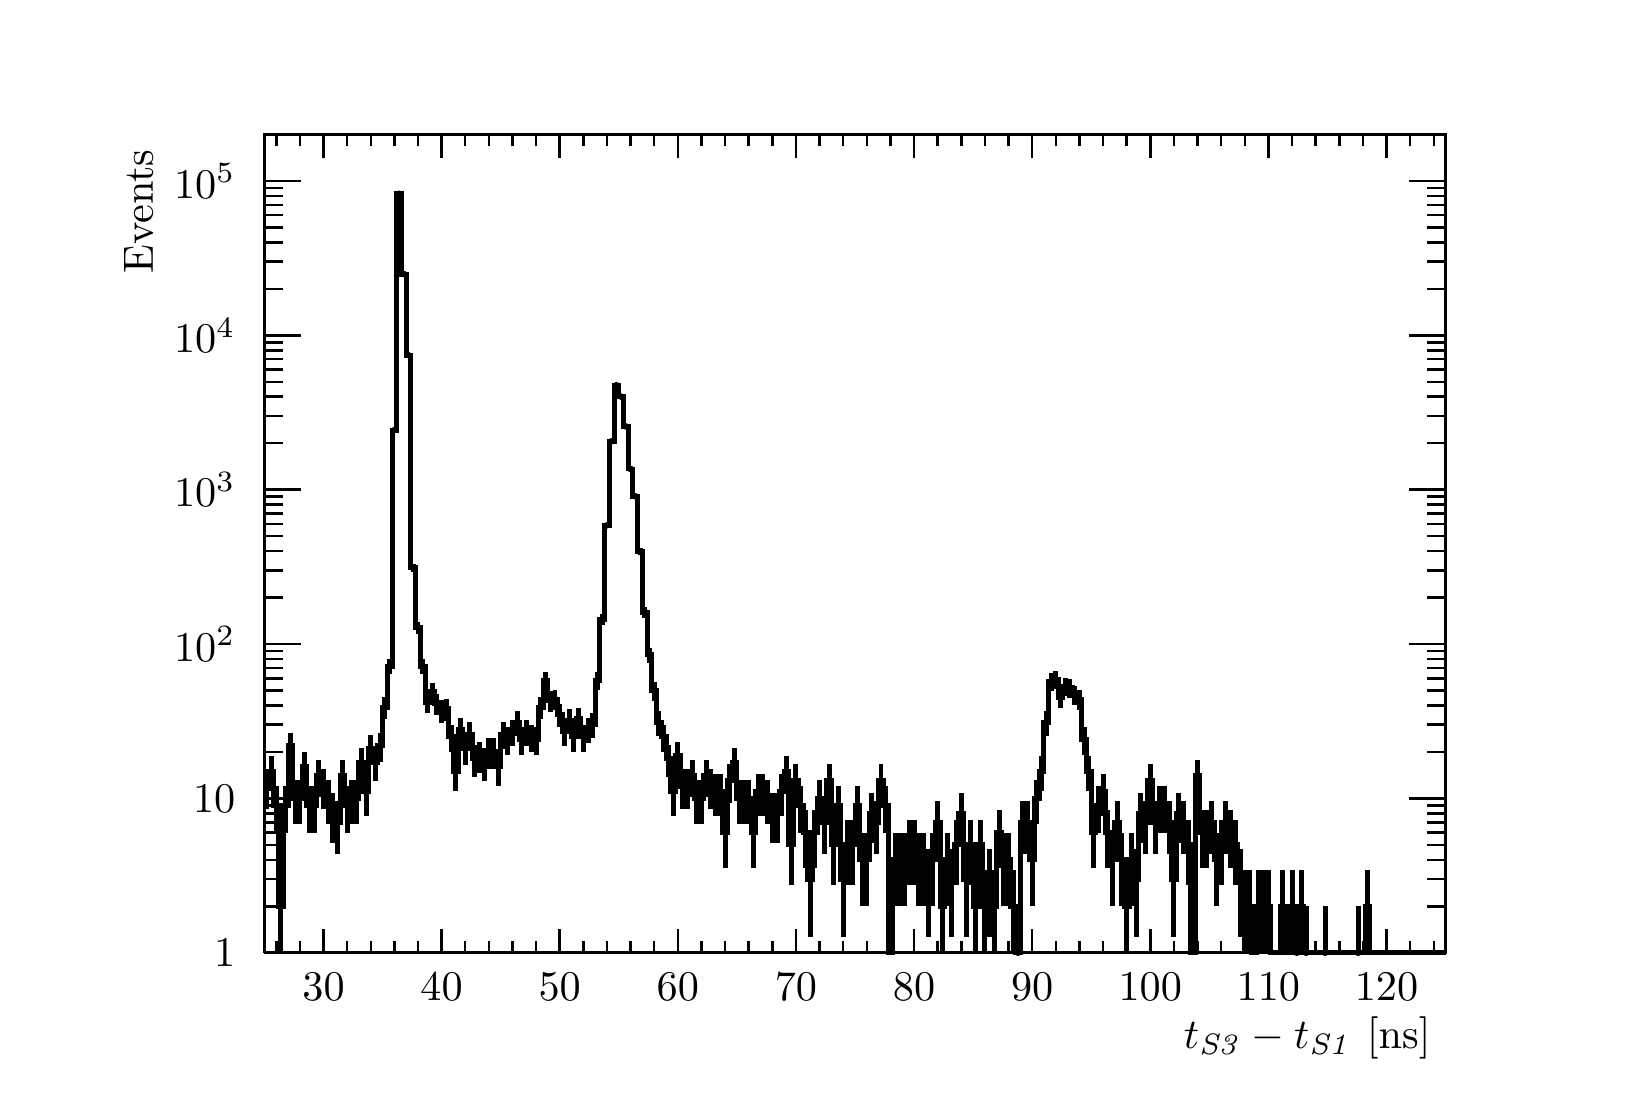
\begin{tikzpicture}
\pgfdeclareplotmark{cross} {
\pgfpathmoveto{\pgfpoint{-0.3\pgfplotmarksize}{\pgfplotmarksize}}
\pgfpathlineto{\pgfpoint{+0.3\pgfplotmarksize}{\pgfplotmarksize}}
\pgfpathlineto{\pgfpoint{+0.3\pgfplotmarksize}{0.3\pgfplotmarksize}}
\pgfpathlineto{\pgfpoint{+1\pgfplotmarksize}{0.3\pgfplotmarksize}}
\pgfpathlineto{\pgfpoint{+1\pgfplotmarksize}{-0.3\pgfplotmarksize}}
\pgfpathlineto{\pgfpoint{+0.3\pgfplotmarksize}{-0.3\pgfplotmarksize}}
\pgfpathlineto{\pgfpoint{+0.3\pgfplotmarksize}{-1.\pgfplotmarksize}}
\pgfpathlineto{\pgfpoint{-0.3\pgfplotmarksize}{-1.\pgfplotmarksize}}
\pgfpathlineto{\pgfpoint{-0.3\pgfplotmarksize}{-0.3\pgfplotmarksize}}
\pgfpathlineto{\pgfpoint{-1.\pgfplotmarksize}{-0.3\pgfplotmarksize}}
\pgfpathlineto{\pgfpoint{-1.\pgfplotmarksize}{0.3\pgfplotmarksize}}
\pgfpathlineto{\pgfpoint{-0.3\pgfplotmarksize}{0.3\pgfplotmarksize}}
\pgfpathclose
\pgfusepathqstroke
}
\pgfdeclareplotmark{cross*} {
\pgfpathmoveto{\pgfpoint{-0.3\pgfplotmarksize}{\pgfplotmarksize}}
\pgfpathlineto{\pgfpoint{+0.3\pgfplotmarksize}{\pgfplotmarksize}}
\pgfpathlineto{\pgfpoint{+0.3\pgfplotmarksize}{0.3\pgfplotmarksize}}
\pgfpathlineto{\pgfpoint{+1\pgfplotmarksize}{0.3\pgfplotmarksize}}
\pgfpathlineto{\pgfpoint{+1\pgfplotmarksize}{-0.3\pgfplotmarksize}}
\pgfpathlineto{\pgfpoint{+0.3\pgfplotmarksize}{-0.3\pgfplotmarksize}}
\pgfpathlineto{\pgfpoint{+0.3\pgfplotmarksize}{-1.\pgfplotmarksize}}
\pgfpathlineto{\pgfpoint{-0.3\pgfplotmarksize}{-1.\pgfplotmarksize}}
\pgfpathlineto{\pgfpoint{-0.3\pgfplotmarksize}{-0.3\pgfplotmarksize}}
\pgfpathlineto{\pgfpoint{-1.\pgfplotmarksize}{-0.3\pgfplotmarksize}}
\pgfpathlineto{\pgfpoint{-1.\pgfplotmarksize}{0.3\pgfplotmarksize}}
\pgfpathlineto{\pgfpoint{-0.3\pgfplotmarksize}{0.3\pgfplotmarksize}}
\pgfpathclose
\pgfusepathqfillstroke
}
\pgfdeclareplotmark{newstar} {
\pgfpathmoveto{\pgfqpoint{0pt}{\pgfplotmarksize}}
\pgfpathlineto{\pgfqpointpolar{44}{0.5\pgfplotmarksize}}
\pgfpathlineto{\pgfqpointpolar{18}{\pgfplotmarksize}}
\pgfpathlineto{\pgfqpointpolar{-20}{0.5\pgfplotmarksize}}
\pgfpathlineto{\pgfqpointpolar{-54}{\pgfplotmarksize}}
\pgfpathlineto{\pgfqpointpolar{-90}{0.5\pgfplotmarksize}}
\pgfpathlineto{\pgfqpointpolar{234}{\pgfplotmarksize}}
\pgfpathlineto{\pgfqpointpolar{198}{0.5\pgfplotmarksize}}
\pgfpathlineto{\pgfqpointpolar{162}{\pgfplotmarksize}}
\pgfpathlineto{\pgfqpointpolar{134}{0.5\pgfplotmarksize}}
\pgfpathclose
\pgfusepathqstroke
}
\pgfdeclareplotmark{newstar*} {
\pgfpathmoveto{\pgfqpoint{0pt}{\pgfplotmarksize}}
\pgfpathlineto{\pgfqpointpolar{44}{0.5\pgfplotmarksize}}
\pgfpathlineto{\pgfqpointpolar{18}{\pgfplotmarksize}}
\pgfpathlineto{\pgfqpointpolar{-20}{0.5\pgfplotmarksize}}
\pgfpathlineto{\pgfqpointpolar{-54}{\pgfplotmarksize}}
\pgfpathlineto{\pgfqpointpolar{-90}{0.5\pgfplotmarksize}}
\pgfpathlineto{\pgfqpointpolar{234}{\pgfplotmarksize}}
\pgfpathlineto{\pgfqpointpolar{198}{0.5\pgfplotmarksize}}
\pgfpathlineto{\pgfqpointpolar{162}{\pgfplotmarksize}}
\pgfpathlineto{\pgfqpointpolar{134}{0.5\pgfplotmarksize}}
\pgfpathclose
\pgfusepathqfillstroke
}
\definecolor{c}{rgb}{1,1,1};
\draw [color=c, fill=c] (0,0) rectangle (20,13.4957);
\draw [color=c, fill=c] (3,1.75444) rectangle (18,12.1461);
\definecolor{c}{rgb}{0,0,0};
\draw [c,line width=0.9] (3,1.75444) -- (3,12.1461) -- (18,12.1461) -- (18,1.75444) -- (3,1.75444);
\definecolor{c}{rgb}{1,1,1};
\draw [color=c, fill=c] (3,1.75444) rectangle (18,12.1461);
\definecolor{c}{rgb}{0,0,0};
\draw [c,line width=0.9] (3,1.75444) -- (3,12.1461) -- (18,12.1461) -- (18,1.75444) -- (3,1.75444);
\draw [c,line width=1.8] (3.03,3.57998) -- (3.03,3.86998);
\draw [c,line width=1.8] (3.03,3.86998) -- (3.03,4.08589);
\foreach \P in {(3.03,3.86998)}{\draw[mark options={color=c,fill=c},mark size=2.402402pt,mark=*,mark size=1pt] plot coordinates {\P};}
\draw [c,line width=1.8] (3.09,3.80567) -- (3.09,4.05995);
\draw [c,line width=1.8] (3.09,4.05995) -- (3.09,4.25549);
\foreach \P in {(3.09,4.05995)}{\draw[mark options={color=c,fill=c},mark size=2.402402pt,mark=*,mark size=1pt] plot coordinates {\P};}
\draw [c,line width=1.8] (3.15,3.27986) -- (3.15,3.62506);
\draw [c,line width=1.8] (3.15,3.62506) -- (3.15,3.86998);
\foreach \P in {(3.15,3.62506)}{\draw[mark options={color=c,fill=c},mark size=2.402402pt,mark=*,mark size=1pt] plot coordinates {\P};}
\draw [c,line width=1.8] (3.21,1.75444) -- (3.21,2.34455);
\draw [c,line width=1.8] (3.21,2.34455) -- (3.21,2.79986);
\foreach \P in {(3.21,2.34455)}{\draw[mark options={color=c,fill=c},mark size=2.402402pt,mark=*,mark size=1pt] plot coordinates {\P};}
\draw [c,line width=1.8] (3.27,3.27986) -- (3.27,3.62506);
\draw [c,line width=1.8] (3.27,3.62506) -- (3.27,3.86998);
\foreach \P in {(3.27,3.62506)}{\draw[mark options={color=c,fill=c},mark size=2.402402pt,mark=*,mark size=1pt] plot coordinates {\P};}
\draw [c,line width=1.8] (3.33,4.18187) -- (3.33,4.38601);
\draw [c,line width=1.8] (3.33,4.38601) -- (3.33,4.55055);
\foreach \P in {(3.33,4.38601)}{\draw[mark options={color=c,fill=c},mark size=2.402402pt,mark=*,mark size=1pt] plot coordinates {\P};}
\draw [c,line width=1.8] (3.39,3.39113) -- (3.39,3.71476);
\draw [c,line width=1.8] (3.39,3.71476) -- (3.39,3.94868);
\foreach \P in {(3.39,3.71476)}{\draw[mark options={color=c,fill=c},mark size=2.402402pt,mark=*,mark size=1pt] plot coordinates {\P};}
\draw [c,line width=1.8] (3.45,3.39113) -- (3.45,3.71476);
\draw [c,line width=1.8] (3.45,3.71476) -- (3.45,3.94868);
\foreach \P in {(3.45,3.71476)}{\draw[mark options={color=c,fill=c},mark size=2.402402pt,mark=*,mark size=1pt] plot coordinates {\P};}
\draw [c,line width=1.8] (3.51,3.86998) -- (3.51,4.1149);
\draw [c,line width=1.8] (3.51,4.1149) -- (3.51,4.30487);
\foreach \P in {(3.51,4.1149)}{\draw[mark options={color=c,fill=c},mark size=2.402402pt,mark=*,mark size=1pt] plot coordinates {\P};}
\draw [c,line width=1.8] (3.57,3.27986) -- (3.57,3.62506);
\draw [c,line width=1.8] (3.57,3.62506) -- (3.57,3.86998);
\foreach \P in {(3.57,3.62506)}{\draw[mark options={color=c,fill=c},mark size=2.402402pt,mark=*,mark size=1pt] plot coordinates {\P};}
\draw [c,line width=1.8] (3.63,3.27986) -- (3.63,3.62506);
\draw [c,line width=1.8] (3.63,3.62506) -- (3.63,3.86998);
\foreach \P in {(3.63,3.62506)}{\draw[mark options={color=c,fill=c},mark size=2.402402pt,mark=*,mark size=1pt] plot coordinates {\P};}
\draw [c,line width=1.8] (3.69,3.73647) -- (3.69,4.00121);
\draw [c,line width=1.8] (3.69,4.00121) -- (3.69,4.20286);
\foreach \P in {(3.69,4.00121)}{\draw[mark options={color=c,fill=c},mark size=2.402402pt,mark=*,mark size=1pt] plot coordinates {\P};}
\draw [c,line width=1.8] (3.75,3.57998) -- (3.75,3.86998);
\draw [c,line width=1.8] (3.75,3.86998) -- (3.75,4.08589);
\foreach \P in {(3.75,3.86998)}{\draw[mark options={color=c,fill=c},mark size=2.402402pt,mark=*,mark size=1pt] plot coordinates {\P};}
\draw [c,line width=1.8] (3.81,3.39113) -- (3.81,3.71476);
\draw [c,line width=1.8] (3.81,3.71476) -- (3.81,3.94868);
\foreach \P in {(3.81,3.71476)}{\draw[mark options={color=c,fill=c},mark size=2.402402pt,mark=*,mark size=1pt] plot coordinates {\P};}
\draw [c,line width=1.8] (3.87,3.15337) -- (3.87,3.52478);
\draw [c,line width=1.8] (3.87,3.52478) -- (3.87,3.78252);
\foreach \P in {(3.87,3.52478)}{\draw[mark options={color=c,fill=c},mark size=2.402402pt,mark=*,mark size=1pt] plot coordinates {\P};}
\draw [c,line width=1.8] (3.93,3.00691) -- (3.93,3.4111);
\draw [c,line width=1.8] (3.93,3.4111) -- (3.93,3.68405);
\foreach \P in {(3.93,3.4111)}{\draw[mark options={color=c,fill=c},mark size=2.402402pt,mark=*,mark size=1pt] plot coordinates {\P};}
\draw [c,line width=1.8] (3.99,3.73647) -- (3.99,4.00121);
\draw [c,line width=1.8] (3.99,4.00121) -- (3.99,4.20286);
\foreach \P in {(3.99,4.00121)}{\draw[mark options={color=c,fill=c},mark size=2.402402pt,mark=*,mark size=1pt] plot coordinates {\P};}
\draw [c,line width=1.8] (4.05,3.27986) -- (4.05,3.62506);
\draw [c,line width=1.8] (4.05,3.62506) -- (4.05,3.86998);
\foreach \P in {(4.05,3.62506)}{\draw[mark options={color=c,fill=c},mark size=2.402402pt,mark=*,mark size=1pt] plot coordinates {\P};}
\draw [c,line width=1.8] (4.11,3.39113) -- (4.11,3.71476);
\draw [c,line width=1.8] (4.11,3.71476) -- (4.11,3.94868);
\foreach \P in {(4.11,3.71476)}{\draw[mark options={color=c,fill=c},mark size=2.402402pt,mark=*,mark size=1pt] plot coordinates {\P};}
\draw [c,line width=1.8] (4.17,3.39113) -- (4.17,3.71476);
\draw [c,line width=1.8] (4.17,3.71476) -- (4.17,3.94868);
\foreach \P in {(4.17,3.71476)}{\draw[mark options={color=c,fill=c},mark size=2.402402pt,mark=*,mark size=1pt] plot coordinates {\P};}
\draw [c,line width=1.8] (4.23,3.93002) -- (4.23,4.16651);
\draw [c,line width=1.8] (4.23,4.16651) -- (4.23,4.35138);
\foreach \P in {(4.23,4.16651)}{\draw[mark options={color=c,fill=c},mark size=2.402402pt,mark=*,mark size=1pt] plot coordinates {\P};}
\draw [c,line width=1.8] (4.29,3.4904) -- (4.29,3.7959);
\draw [c,line width=1.8] (4.29,3.7959) -- (4.29,4.02025);
\foreach \P in {(4.29,3.7959)}{\draw[mark options={color=c,fill=c},mark size=2.402402pt,mark=*,mark size=1pt] plot coordinates {\P};}
\draw [c,line width=1.8] (4.35,4.13682) -- (4.35,4.34641);
\draw [c,line width=1.8] (4.35,4.34641) -- (4.35,4.51446);
\foreach \P in {(4.35,4.34641)}{\draw[mark options={color=c,fill=c},mark size=2.402402pt,mark=*,mark size=1pt] plot coordinates {\P};}
\draw [c,line width=1.8] (4.41,3.93002) -- (4.41,4.16651);
\draw [c,line width=1.8] (4.41,4.16651) -- (4.41,4.35138);
\foreach \P in {(4.41,4.16651)}{\draw[mark options={color=c,fill=c},mark size=2.402402pt,mark=*,mark size=1pt] plot coordinates {\P};}
\draw [c,line width=1.8] (4.47,4.18187) -- (4.47,4.38601);
\draw [c,line width=1.8] (4.47,4.38601) -- (4.47,4.55055);
\foreach \P in {(4.47,4.38601)}{\draw[mark options={color=c,fill=c},mark size=2.402402pt,mark=*,mark size=1pt] plot coordinates {\P};}
\draw [c,line width=1.8] (4.53,4.72486) -- (4.53,4.87343);
\draw [c,line width=1.8] (4.53,4.87343) -- (4.53,4.99988);
\foreach \P in {(4.53,4.87343)}{\draw[mark options={color=c,fill=c},mark size=2.402402pt,mark=*,mark size=1pt] plot coordinates {\P};}
\draw [c,line width=1.8] (4.59,5.28864) -- (4.59,5.3954);
\draw [c,line width=1.8] (4.59,5.3954) -- (4.59,5.49025);
\foreach \P in {(4.59,5.3954)}{\draw[mark options={color=c,fill=c},mark size=2.402402pt,mark=*,mark size=1pt] plot coordinates {\P};}
\draw [c,line width=1.8] (4.65,8.3742) -- (4.65,8.39165);
\draw [c,line width=1.8] (4.65,8.39165) -- (4.65,8.40874);
\foreach \P in {(4.65,8.39165)}{\draw[mark options={color=c,fill=c},mark size=2.402402pt,mark=*,mark size=1pt] plot coordinates {\P};}
\draw [c,line width=1.8] (4.71,11.3894) -- (4.71,11.3924);
\draw [c,line width=1.8] (4.71,11.3924) -- (4.71,11.3953);
\foreach \P in {(4.71,11.3924)}{\draw[mark options={color=c,fill=c},mark size=2.402402pt,mark=*,mark size=1pt] plot coordinates {\P};}
\draw [c,line width=1.8] (4.77,10.3684) -- (4.77,10.3738);
\draw [c,line width=1.8] (4.77,10.3738) -- (4.77,10.3792);
\foreach \P in {(4.77,10.3738)}{\draw[mark options={color=c,fill=c},mark size=2.402402pt,mark=*,mark size=1pt] plot coordinates {\P};}
\draw [c,line width=1.8] (4.83,9.33206) -- (4.83,9.342);
\draw [c,line width=1.8] (4.83,9.342) -- (4.83,9.35182);
\foreach \P in {(4.83,9.342)}{\draw[mark options={color=c,fill=c},mark size=2.402402pt,mark=*,mark size=1pt] plot coordinates {\P};}
\draw [c,line width=1.8] (4.89,6.59134) -- (4.89,6.64104);
\draw [c,line width=1.8] (4.89,6.64104) -- (4.89,6.68799);
\foreach \P in {(4.89,6.64104)}{\draw[mark options={color=c,fill=c},mark size=2.402402pt,mark=*,mark size=1pt] plot coordinates {\P};}
\draw [c,line width=1.8] (4.95,5.80645) -- (4.95,5.88524);
\draw [c,line width=1.8] (4.95,5.88524) -- (4.95,5.95735);
\foreach \P in {(4.95,5.88524)}{\draw[mark options={color=c,fill=c},mark size=2.402402pt,mark=*,mark size=1pt] plot coordinates {\P};}
\draw [c,line width=1.8] (5.01,5.28864) -- (5.01,5.3954);
\draw [c,line width=1.8] (5.01,5.3954) -- (5.01,5.49025);
\foreach \P in {(5.01,5.3954)}{\draw[mark options={color=c,fill=c},mark size=2.402402pt,mark=*,mark size=1pt] plot coordinates {\P};}
\draw [c,line width=1.8] (5.07,4.79384) -- (5.07,4.93652);
\draw [c,line width=1.8] (5.07,4.93652) -- (5.07,5.05869);
\foreach \P in {(5.07,4.93652)}{\draw[mark options={color=c,fill=c},mark size=2.402402pt,mark=*,mark size=1pt] plot coordinates {\P};}
\draw [c,line width=1.8] (5.13,4.93652) -- (5.13,5.06776);
\draw [c,line width=1.8] (5.13,5.06776) -- (5.13,5.18144);
\foreach \P in {(5.13,5.06776)}{\draw[mark options={color=c,fill=c},mark size=2.402402pt,mark=*,mark size=1pt] plot coordinates {\P};}
\draw [c,line width=1.8] (5.19,4.77144) -- (5.19,4.91601);
\draw [c,line width=1.8] (5.19,4.91601) -- (5.19,5.03955);
\foreach \P in {(5.19,4.91601)}{\draw[mark options={color=c,fill=c},mark size=2.402402pt,mark=*,mark size=1pt] plot coordinates {\P};}
\draw [c,line width=1.8] (5.25,4.6757) -- (5.25,4.82861);
\draw [c,line width=1.8] (5.25,4.82861) -- (5.25,4.95819);
\foreach \P in {(5.25,4.82861)}{\draw[mark options={color=c,fill=c},mark size=2.402402pt,mark=*,mark size=1pt] plot coordinates {\P};}
\draw [c,line width=1.8] (5.31,4.70062) -- (5.31,4.85132);
\draw [c,line width=1.8] (5.31,4.85132) -- (5.31,4.9793);
\foreach \P in {(5.31,4.85132)}{\draw[mark options={color=c,fill=c},mark size=2.402402pt,mark=*,mark size=1pt] plot coordinates {\P};}
\draw [c,line width=1.8] (5.37,4.30487) -- (5.37,4.49484);
\draw [c,line width=1.8] (5.37,4.49484) -- (5.37,4.65006);
\foreach \P in {(5.37,4.49484)}{\draw[mark options={color=c,fill=c},mark size=2.402402pt,mark=*,mark size=1pt] plot coordinates {\P};}
\draw [c,line width=1.8] (5.43,3.80567) -- (5.43,4.05995);
\draw [c,line width=1.8] (5.43,4.05995) -- (5.43,4.25549);
\foreach \P in {(5.43,4.05995)}{\draw[mark options={color=c,fill=c},mark size=2.402402pt,mark=*,mark size=1pt] plot coordinates {\P};}
\draw [c,line width=1.8] (5.49,4.413) -- (5.49,4.59133);
\draw [c,line width=1.8] (5.49,4.59133) -- (5.49,4.73869);
\foreach \P in {(5.49,4.59133)}{\draw[mark options={color=c,fill=c},mark size=2.402402pt,mark=*,mark size=1pt] plot coordinates {\P};}
\draw [c,line width=1.8] (5.55,4.13682) -- (5.55,4.34641);
\draw [c,line width=1.8] (5.55,4.34641) -- (5.55,4.51446);
\foreach \P in {(5.55,4.34641)}{\draw[mark options={color=c,fill=c},mark size=2.402402pt,mark=*,mark size=1pt] plot coordinates {\P};}
\draw [c,line width=1.8] (5.61,4.34238) -- (5.61,4.52823);
\draw [c,line width=1.8] (5.61,4.52823) -- (5.61,4.6807);
\foreach \P in {(5.61,4.52823)}{\draw[mark options={color=c,fill=c},mark size=2.402402pt,mark=*,mark size=1pt] plot coordinates {\P};}
\draw [c,line width=1.8] (5.67,3.98633) -- (5.67,4.21517);
\draw [c,line width=1.8] (5.67,4.21517) -- (5.67,4.39535);
\foreach \P in {(5.67,4.21517)}{\draw[mark options={color=c,fill=c},mark size=2.402402pt,mark=*,mark size=1pt] plot coordinates {\P};}
\draw [c,line width=1.8] (5.73,4.03933) -- (5.73,4.2612);
\draw [c,line width=1.8] (5.73,4.2612) -- (5.73,4.43704);
\foreach \P in {(5.73,4.2612)}{\draw[mark options={color=c,fill=c},mark size=2.402402pt,mark=*,mark size=1pt] plot coordinates {\P};}
\draw [c,line width=1.8] (5.79,3.93002) -- (5.79,4.16651);
\draw [c,line width=1.8] (5.79,4.16651) -- (5.79,4.35138);
\foreach \P in {(5.79,4.16651)}{\draw[mark options={color=c,fill=c},mark size=2.402402pt,mark=*,mark size=1pt] plot coordinates {\P};}
\draw [c,line width=1.8] (5.85,4.0894) -- (5.85,4.30487);
\draw [c,line width=1.8] (5.85,4.30487) -- (5.85,4.47668);
\foreach \P in {(5.85,4.30487)}{\draw[mark options={color=c,fill=c},mark size=2.402402pt,mark=*,mark size=1pt] plot coordinates {\P};}
\draw [c,line width=1.8] (5.91,4.0894) -- (5.91,4.30487);
\draw [c,line width=1.8] (5.91,4.30487) -- (5.91,4.47668);
\foreach \P in {(5.91,4.30487)}{\draw[mark options={color=c,fill=c},mark size=2.402402pt,mark=*,mark size=1pt] plot coordinates {\P};}
\draw [c,line width=1.8] (5.97,3.86998) -- (5.97,4.1149);
\draw [c,line width=1.8] (5.97,4.1149) -- (5.97,4.30487);
\foreach \P in {(5.97,4.1149)}{\draw[mark options={color=c,fill=c},mark size=2.402402pt,mark=*,mark size=1pt] plot coordinates {\P};}
\draw [c,line width=1.8] (6.03,4.34238) -- (6.03,4.52823);
\draw [c,line width=1.8] (6.03,4.52823) -- (6.03,4.6807);
\foreach \P in {(6.03,4.52823)}{\draw[mark options={color=c,fill=c},mark size=2.402402pt,mark=*,mark size=1pt] plot coordinates {\P};}
\draw [c,line width=1.8] (6.09,4.26572) -- (6.09,4.46009);
\draw [c,line width=1.8] (6.09,4.46009) -- (6.09,4.61823);
\foreach \P in {(6.09,4.46009)}{\draw[mark options={color=c,fill=c},mark size=2.402402pt,mark=*,mark size=1pt] plot coordinates {\P};}
\draw [c,line width=1.8] (6.15,4.37839) -- (6.15,4.56037);
\draw [c,line width=1.8] (6.15,4.56037) -- (6.15,4.71021);
\foreach \P in {(6.15,4.56037)}{\draw[mark options={color=c,fill=c},mark size=2.402402pt,mark=*,mark size=1pt] plot coordinates {\P};}
\draw [c,line width=1.8] (6.21,4.50944) -- (6.21,4.67798);
\draw [c,line width=1.8] (6.21,4.67798) -- (6.21,4.81861);
\foreach \P in {(6.21,4.67798)}{\draw[mark options={color=c,fill=c},mark size=2.402402pt,mark=*,mark size=1pt] plot coordinates {\P};}
\draw [c,line width=1.8] (6.27,4.26572) -- (6.27,4.46009);
\draw [c,line width=1.8] (6.27,4.46009) -- (6.27,4.61823);
\foreach \P in {(6.27,4.46009)}{\draw[mark options={color=c,fill=c},mark size=2.402402pt,mark=*,mark size=1pt] plot coordinates {\P};}
\draw [c,line width=1.8] (6.33,4.37839) -- (6.33,4.56037);
\draw [c,line width=1.8] (6.33,4.56037) -- (6.33,4.71021);
\foreach \P in {(6.33,4.56037)}{\draw[mark options={color=c,fill=c},mark size=2.402402pt,mark=*,mark size=1pt] plot coordinates {\P};}
\draw [c,line width=1.8] (6.39,4.30487) -- (6.39,4.49484);
\draw [c,line width=1.8] (6.39,4.49484) -- (6.39,4.65006);
\foreach \P in {(6.39,4.49484)}{\draw[mark options={color=c,fill=c},mark size=2.402402pt,mark=*,mark size=1pt] plot coordinates {\P};}
\draw [c,line width=1.8] (6.45,4.26572) -- (6.45,4.46009);
\draw [c,line width=1.8] (6.45,4.46009) -- (6.45,4.61823);
\foreach \P in {(6.45,4.46009)}{\draw[mark options={color=c,fill=c},mark size=2.402402pt,mark=*,mark size=1pt] plot coordinates {\P};}
\draw [c,line width=1.8] (6.51,4.72486) -- (6.51,4.87343);
\draw [c,line width=1.8] (6.51,4.87343) -- (6.51,4.99988);
\foreach \P in {(6.51,4.87343)}{\draw[mark options={color=c,fill=c},mark size=2.402402pt,mark=*,mark size=1pt] plot coordinates {\P};}
\draw [c,line width=1.8] (6.57,5.09148) -- (6.57,5.21132);
\draw [c,line width=1.8] (6.57,5.21132) -- (6.57,5.31635);
\foreach \P in {(6.57,5.21132)}{\draw[mark options={color=c,fill=c},mark size=2.402402pt,mark=*,mark size=1pt] plot coordinates {\P};}
\draw [c,line width=1.8] (6.63,4.81569) -- (6.63,4.95655);
\draw [c,line width=1.8] (6.63,4.95655) -- (6.63,5.07739);
\foreach \P in {(6.63,4.95655)}{\draw[mark options={color=c,fill=c},mark size=2.402402pt,mark=*,mark size=1pt] plot coordinates {\P};}
\draw [c,line width=1.8] (6.69,4.83701) -- (6.69,4.97613);
\draw [c,line width=1.8] (6.69,4.97613) -- (6.69,5.09567);
\foreach \P in {(6.69,4.97613)}{\draw[mark options={color=c,fill=c},mark size=2.402402pt,mark=*,mark size=1pt] plot coordinates {\P};}
\draw [c,line width=1.8] (6.75,4.62366) -- (6.75,4.7813);
\draw [c,line width=1.8] (6.75,4.7813) -- (6.75,4.91426);
\foreach \P in {(6.75,4.7813)}{\draw[mark options={color=c,fill=c},mark size=2.402402pt,mark=*,mark size=1pt] plot coordinates {\P};}
\draw [c,line width=1.8] (6.81,4.37839) -- (6.81,4.56037);
\draw [c,line width=1.8] (6.81,4.56037) -- (6.81,4.71021);
\foreach \P in {(6.81,4.56037)}{\draw[mark options={color=c,fill=c},mark size=2.402402pt,mark=*,mark size=1pt] plot coordinates {\P};}
\draw [c,line width=1.8] (6.87,4.5394) -- (6.87,4.70501);
\draw [c,line width=1.8] (6.87,4.70501) -- (6.87,4.84359);
\foreach \P in {(6.87,4.70501)}{\draw[mark options={color=c,fill=c},mark size=2.402402pt,mark=*,mark size=1pt] plot coordinates {\P};}
\draw [c,line width=1.8] (6.93,4.30487) -- (6.93,4.49484);
\draw [c,line width=1.8] (6.93,4.49484) -- (6.93,4.65006);
\foreach \P in {(6.93,4.49484)}{\draw[mark options={color=c,fill=c},mark size=2.402402pt,mark=*,mark size=1pt] plot coordinates {\P};}
\draw [c,line width=1.8] (6.99,4.56838) -- (6.99,4.73121);
\draw [c,line width=1.8] (6.99,4.73121) -- (6.99,4.86784);
\foreach \P in {(6.99,4.73121)}{\draw[mark options={color=c,fill=c},mark size=2.402402pt,mark=*,mark size=1pt] plot coordinates {\P};}
\draw [c,line width=1.8] (7.05,4.30487) -- (7.05,4.49484);
\draw [c,line width=1.8] (7.05,4.49484) -- (7.05,4.65006);
\foreach \P in {(7.05,4.49484)}{\draw[mark options={color=c,fill=c},mark size=2.402402pt,mark=*,mark size=1pt] plot coordinates {\P};}
\draw [c,line width=1.8] (7.11,4.413) -- (7.11,4.59133);
\draw [c,line width=1.8] (7.11,4.59133) -- (7.11,4.73869);
\foreach \P in {(7.11,4.59133)}{\draw[mark options={color=c,fill=c},mark size=2.402402pt,mark=*,mark size=1pt] plot coordinates {\P};}
\draw [c,line width=1.8] (7.17,4.47844) -- (7.17,4.65006);
\draw [c,line width=1.8] (7.17,4.65006) -- (7.17,4.79283);
\foreach \P in {(7.17,4.65006)}{\draw[mark options={color=c,fill=c},mark size=2.402402pt,mark=*,mark size=1pt] plot coordinates {\P};}
\draw [c,line width=1.8] (7.23,5.09148) -- (7.23,5.21132);
\draw [c,line width=1.8] (7.23,5.21132) -- (7.23,5.31635);
\foreach \P in {(7.23,5.21132)}{\draw[mark options={color=c,fill=c},mark size=2.402402pt,mark=*,mark size=1pt] plot coordinates {\P};}
\draw [c,line width=1.8] (7.29,5.91759) -- (7.29,5.9914);
\draw [c,line width=1.8] (7.29,5.9914) -- (7.29,6.05932);
\foreach \P in {(7.29,5.9914)}{\draw[mark options={color=c,fill=c},mark size=2.402402pt,mark=*,mark size=1pt] plot coordinates {\P};}
\draw [c,line width=1.8] (7.35,7.14744) -- (7.35,7.18329);
\draw [c,line width=1.8] (7.35,7.18329) -- (7.35,7.2177);
\foreach \P in {(7.35,7.18329)}{\draw[mark options={color=c,fill=c},mark size=2.402402pt,mark=*,mark size=1pt] plot coordinates {\P};}
\draw [c,line width=1.8] (7.41,8.23044) -- (7.41,8.24942);
\draw [c,line width=1.8] (7.41,8.24942) -- (7.41,8.26799);
\foreach \P in {(7.41,8.24942)}{\draw[mark options={color=c,fill=c},mark size=2.402402pt,mark=*,mark size=1pt] plot coordinates {\P};}
\draw [c,line width=1.8] (7.47,8.9493) -- (7.47,8.96174);
\draw [c,line width=1.8] (7.47,8.96174) -- (7.47,8.97401);
\foreach \P in {(7.47,8.96174)}{\draw[mark options={color=c,fill=c},mark size=2.402402pt,mark=*,mark size=1pt] plot coordinates {\P};}
\draw [c,line width=1.8] (7.53,8.80269) -- (7.53,8.81625);
\draw [c,line width=1.8] (7.53,8.81625) -- (7.53,8.8296);
\foreach \P in {(7.53,8.81625)}{\draw[mark options={color=c,fill=c},mark size=2.402402pt,mark=*,mark size=1pt] plot coordinates {\P};}
\draw [c,line width=1.8] (7.59,8.42169) -- (7.59,8.43865);
\draw [c,line width=1.8] (7.59,8.43865) -- (7.59,8.45529);
\foreach \P in {(7.59,8.43865)}{\draw[mark options={color=c,fill=c},mark size=2.402402pt,mark=*,mark size=1pt] plot coordinates {\P};}
\draw [c,line width=1.8] (7.65,7.8744) -- (7.65,7.89779);
\draw [c,line width=1.8] (7.65,7.89779) -- (7.65,7.92056);
\foreach \P in {(7.65,7.89779)}{\draw[mark options={color=c,fill=c},mark size=2.402402pt,mark=*,mark size=1pt] plot coordinates {\P};}
\draw [c,line width=1.8] (7.71,7.52162) -- (7.71,7.5504);
\draw [c,line width=1.8] (7.71,7.5504) -- (7.71,7.57824);
\foreach \P in {(7.71,7.5504)}{\draw[mark options={color=c,fill=c},mark size=2.402402pt,mark=*,mark size=1pt] plot coordinates {\P};}
\draw [c,line width=1.8] (7.77,6.80285) -- (7.77,6.84674);
\draw [c,line width=1.8] (7.77,6.84674) -- (7.77,6.88848);
\foreach \P in {(7.77,6.84674)}{\draw[mark options={color=c,fill=c},mark size=2.402402pt,mark=*,mark size=1pt] plot coordinates {\P};}
\draw [c,line width=1.8] (7.83,6.01063) -- (7.83,6.08052);
\draw [c,line width=1.8] (7.83,6.08052) -- (7.83,6.1451);
\foreach \P in {(7.83,6.08052)}{\draw[mark options={color=c,fill=c},mark size=2.402402pt,mark=*,mark size=1pt] plot coordinates {\P};}
\draw [c,line width=1.8] (7.89,5.43897) -- (7.89,5.53671);
\draw [c,line width=1.8] (7.89,5.53671) -- (7.89,5.62438);
\foreach \P in {(7.89,5.53671)}{\draw[mark options={color=c,fill=c},mark size=2.402402pt,mark=*,mark size=1pt] plot coordinates {\P};}
\draw [c,line width=1.8] (7.95,4.95515) -- (7.95,5.08496);
\draw [c,line width=1.8] (7.95,5.08496) -- (7.95,5.19757);
\foreach \P in {(7.95,5.08496)}{\draw[mark options={color=c,fill=c},mark size=2.402402pt,mark=*,mark size=1pt] plot coordinates {\P};}
\draw [c,line width=1.8] (8.01,4.50944) -- (8.01,4.67798);
\draw [c,line width=1.8] (8.01,4.67798) -- (8.01,4.81861);
\foreach \P in {(8.01,4.67798)}{\draw[mark options={color=c,fill=c},mark size=2.402402pt,mark=*,mark size=1pt] plot coordinates {\P};}
\draw [c,line width=1.8] (8.07,4.30487) -- (8.07,4.49484);
\draw [c,line width=1.8] (8.07,4.49484) -- (8.07,4.65006);
\foreach \P in {(8.07,4.49484)}{\draw[mark options={color=c,fill=c},mark size=2.402402pt,mark=*,mark size=1pt] plot coordinates {\P};}
\draw [c,line width=1.8] (8.13,3.98633) -- (8.13,4.21517);
\draw [c,line width=1.8] (8.13,4.21517) -- (8.13,4.39535);
\foreach \P in {(8.13,4.21517)}{\draw[mark options={color=c,fill=c},mark size=2.402402pt,mark=*,mark size=1pt] plot coordinates {\P};}
\draw [c,line width=1.8] (8.19,3.4904) -- (8.19,3.7959);
\draw [c,line width=1.8] (8.19,3.7959) -- (8.19,4.02025);
\foreach \P in {(8.19,3.7959)}{\draw[mark options={color=c,fill=c},mark size=2.402402pt,mark=*,mark size=1pt] plot coordinates {\P};}
\draw [c,line width=1.8] (8.25,4.03933) -- (8.25,4.2612);
\draw [c,line width=1.8] (8.25,4.2612) -- (8.25,4.43704);
\foreach \P in {(8.25,4.2612)}{\draw[mark options={color=c,fill=c},mark size=2.402402pt,mark=*,mark size=1pt] plot coordinates {\P};}
\draw [c,line width=1.8] (8.31,3.57998) -- (8.31,3.86998);
\draw [c,line width=1.8] (8.31,3.86998) -- (8.31,4.08589);
\foreach \P in {(8.31,3.86998)}{\draw[mark options={color=c,fill=c},mark size=2.402402pt,mark=*,mark size=1pt] plot coordinates {\P};}
\draw [c,line width=1.8] (8.37,3.57998) -- (8.37,3.86998);
\draw [c,line width=1.8] (8.37,3.86998) -- (8.37,4.08589);
\foreach \P in {(8.37,3.86998)}{\draw[mark options={color=c,fill=c},mark size=2.402402pt,mark=*,mark size=1pt] plot coordinates {\P};}
\draw [c,line width=1.8] (8.43,3.73647) -- (8.43,4.00121);
\draw [c,line width=1.8] (8.43,4.00121) -- (8.43,4.20286);
\foreach \P in {(8.43,4.00121)}{\draw[mark options={color=c,fill=c},mark size=2.402402pt,mark=*,mark size=1pt] plot coordinates {\P};}
\draw [c,line width=1.8] (8.49,3.39113) -- (8.49,3.71476);
\draw [c,line width=1.8] (8.49,3.71476) -- (8.49,3.94868);
\foreach \P in {(8.49,3.71476)}{\draw[mark options={color=c,fill=c},mark size=2.402402pt,mark=*,mark size=1pt] plot coordinates {\P};}
\draw [c,line width=1.8] (8.55,3.39113) -- (8.55,3.71476);
\draw [c,line width=1.8] (8.55,3.71476) -- (8.55,3.94868);
\foreach \P in {(8.55,3.71476)}{\draw[mark options={color=c,fill=c},mark size=2.402402pt,mark=*,mark size=1pt] plot coordinates {\P};}
\draw [c,line width=1.8] (8.61,3.73647) -- (8.61,4.00121);
\draw [c,line width=1.8] (8.61,4.00121) -- (8.61,4.20286);
\foreach \P in {(8.61,4.00121)}{\draw[mark options={color=c,fill=c},mark size=2.402402pt,mark=*,mark size=1pt] plot coordinates {\P};}
\draw [c,line width=1.8] (8.67,3.57998) -- (8.67,3.86998);
\draw [c,line width=1.8] (8.67,3.86998) -- (8.67,4.08589);
\foreach \P in {(8.67,3.86998)}{\draw[mark options={color=c,fill=c},mark size=2.402402pt,mark=*,mark size=1pt] plot coordinates {\P};}
\draw [c,line width=1.8] (8.73,3.4904) -- (8.73,3.7959);
\draw [c,line width=1.8] (8.73,3.7959) -- (8.73,4.02025);
\foreach \P in {(8.73,3.7959)}{\draw[mark options={color=c,fill=c},mark size=2.402402pt,mark=*,mark size=1pt] plot coordinates {\P};}
\draw [c,line width=1.8] (8.79,3.4904) -- (8.79,3.7959);
\draw [c,line width=1.8] (8.79,3.7959) -- (8.79,4.02025);
\foreach \P in {(8.79,3.7959)}{\draw[mark options={color=c,fill=c},mark size=2.402402pt,mark=*,mark size=1pt] plot coordinates {\P};}
\draw [c,line width=1.8] (8.85,2.83318) -- (8.85,3.27986);
\draw [c,line width=1.8] (8.85,3.27986) -- (8.85,3.57132);
\foreach \P in {(8.85,3.27986)}{\draw[mark options={color=c,fill=c},mark size=2.402402pt,mark=*,mark size=1pt] plot coordinates {\P};}
\draw [c,line width=1.8] (8.91,3.66158) -- (8.91,3.93812);
\draw [c,line width=1.8] (8.91,3.93812) -- (8.91,4.14652);
\foreach \P in {(8.91,3.93812)}{\draw[mark options={color=c,fill=c},mark size=2.402402pt,mark=*,mark size=1pt] plot coordinates {\P};}
\draw [c,line width=1.8] (8.97,3.93002) -- (8.97,4.16651);
\draw [c,line width=1.8] (8.97,4.16651) -- (8.97,4.35138);
\foreach \P in {(8.97,4.16651)}{\draw[mark options={color=c,fill=c},mark size=2.402402pt,mark=*,mark size=1pt] plot coordinates {\P};}
\draw [c,line width=1.8] (9.03,3.39113) -- (9.03,3.71476);
\draw [c,line width=1.8] (9.03,3.71476) -- (9.03,3.94868);
\foreach \P in {(9.03,3.71476)}{\draw[mark options={color=c,fill=c},mark size=2.402402pt,mark=*,mark size=1pt] plot coordinates {\P};}
\draw [c,line width=1.8] (9.09,3.39113) -- (9.09,3.71476);
\draw [c,line width=1.8] (9.09,3.71476) -- (9.09,3.94868);
\foreach \P in {(9.09,3.71476)}{\draw[mark options={color=c,fill=c},mark size=2.402402pt,mark=*,mark size=1pt] plot coordinates {\P};}
\draw [c,line width=1.8] (9.15,3.39113) -- (9.15,3.71476);
\draw [c,line width=1.8] (9.15,3.71476) -- (9.15,3.94868);
\foreach \P in {(9.15,3.71476)}{\draw[mark options={color=c,fill=c},mark size=2.402402pt,mark=*,mark size=1pt] plot coordinates {\P};}
\draw [c,line width=1.8] (9.21,2.83318) -- (9.21,3.27986);
\draw [c,line width=1.8] (9.21,3.27986) -- (9.21,3.57132);
\foreach \P in {(9.21,3.27986)}{\draw[mark options={color=c,fill=c},mark size=2.402402pt,mark=*,mark size=1pt] plot coordinates {\P};}
\draw [c,line width=1.8] (9.27,3.4904) -- (9.27,3.7959);
\draw [c,line width=1.8] (9.27,3.7959) -- (9.27,4.02025);
\foreach \P in {(9.27,3.7959)}{\draw[mark options={color=c,fill=c},mark size=2.402402pt,mark=*,mark size=1pt] plot coordinates {\P};}
\draw [c,line width=1.8] (9.33,3.4904) -- (9.33,3.7959);
\draw [c,line width=1.8] (9.33,3.7959) -- (9.33,4.02025);
\foreach \P in {(9.33,3.7959)}{\draw[mark options={color=c,fill=c},mark size=2.402402pt,mark=*,mark size=1pt] plot coordinates {\P};}
\draw [c,line width=1.8] (9.39,3.39113) -- (9.39,3.71476);
\draw [c,line width=1.8] (9.39,3.71476) -- (9.39,3.94868);
\foreach \P in {(9.39,3.71476)}{\draw[mark options={color=c,fill=c},mark size=2.402402pt,mark=*,mark size=1pt] plot coordinates {\P};}
\draw [c,line width=1.8] (9.45,3.15337) -- (9.45,3.52478);
\draw [c,line width=1.8] (9.45,3.52478) -- (9.45,3.78252);
\foreach \P in {(9.45,3.52478)}{\draw[mark options={color=c,fill=c},mark size=2.402402pt,mark=*,mark size=1pt] plot coordinates {\P};}
\draw [c,line width=1.8] (9.51,3.15337) -- (9.51,3.52478);
\draw [c,line width=1.8] (9.51,3.52478) -- (9.51,3.78252);
\foreach \P in {(9.51,3.52478)}{\draw[mark options={color=c,fill=c},mark size=2.402402pt,mark=*,mark size=1pt] plot coordinates {\P};}
\draw [c,line width=1.8] (9.57,3.4904) -- (9.57,3.7959);
\draw [c,line width=1.8] (9.57,3.7959) -- (9.57,4.02025);
\foreach \P in {(9.57,3.7959)}{\draw[mark options={color=c,fill=c},mark size=2.402402pt,mark=*,mark size=1pt] plot coordinates {\P};}
\draw [c,line width=1.8] (9.63,3.80567) -- (9.63,4.05995);
\draw [c,line width=1.8] (9.63,4.05995) -- (9.63,4.25549);
\foreach \P in {(9.63,4.05995)}{\draw[mark options={color=c,fill=c},mark size=2.402402pt,mark=*,mark size=1pt] plot coordinates {\P};}
\draw [c,line width=1.8] (9.69,2.61997) -- (9.69,3.12464);
\draw [c,line width=1.8] (9.69,3.12464) -- (9.69,3.43934);
\foreach \P in {(9.69,3.12464)}{\draw[mark options={color=c,fill=c},mark size=2.402402pt,mark=*,mark size=1pt] plot coordinates {\P};}
\draw [c,line width=1.8] (9.75,3.66158) -- (9.75,3.93812);
\draw [c,line width=1.8] (9.75,3.93812) -- (9.75,4.14652);
\foreach \P in {(9.75,3.93812)}{\draw[mark options={color=c,fill=c},mark size=2.402402pt,mark=*,mark size=1pt] plot coordinates {\P};}
\draw [c,line width=1.8] (9.81,3.27986) -- (9.81,3.62506);
\draw [c,line width=1.8] (9.81,3.62506) -- (9.81,3.86998);
\foreach \P in {(9.81,3.62506)}{\draw[mark options={color=c,fill=c},mark size=2.402402pt,mark=*,mark size=1pt] plot coordinates {\P};}
\draw [c,line width=1.8] (9.87,2.83318) -- (9.87,3.27986);
\draw [c,line width=1.8] (9.87,3.27986) -- (9.87,3.57132);
\foreach \P in {(9.87,3.27986)}{\draw[mark options={color=c,fill=c},mark size=2.402402pt,mark=*,mark size=1pt] plot coordinates {\P};}
\draw [c,line width=1.8] (9.93,1.95655) -- (9.93,2.68975);
\draw [c,line width=1.8] (9.93,2.68975) -- (9.93,3.07775);
\foreach \P in {(9.93,2.68975)}{\draw[mark options={color=c,fill=c},mark size=2.402402pt,mark=*,mark size=1pt] plot coordinates {\P};}
\draw [c,line width=1.8] (9.99,2.83318) -- (9.99,3.27986);
\draw [c,line width=1.8] (9.99,3.27986) -- (9.99,3.57132);
\foreach \P in {(9.99,3.27986)}{\draw[mark options={color=c,fill=c},mark size=2.402402pt,mark=*,mark size=1pt] plot coordinates {\P};}
\draw [c,line width=1.8] (10.05,3.39113) -- (10.05,3.71476);
\draw [c,line width=1.8] (10.05,3.71476) -- (10.05,3.94868);
\foreach \P in {(10.05,3.71476)}{\draw[mark options={color=c,fill=c},mark size=2.402402pt,mark=*,mark size=1pt] plot coordinates {\P};}
\draw [c,line width=1.8] (10.11,3.00691) -- (10.11,3.4111);
\draw [c,line width=1.8] (10.11,3.4111) -- (10.11,3.68405);
\foreach \P in {(10.11,3.4111)}{\draw[mark options={color=c,fill=c},mark size=2.402402pt,mark=*,mark size=1pt] plot coordinates {\P};}
\draw [c,line width=1.8] (10.17,3.66158) -- (10.17,3.93812);
\draw [c,line width=1.8] (10.17,3.93812) -- (10.17,4.14652);
\foreach \P in {(10.17,3.93812)}{\draw[mark options={color=c,fill=c},mark size=2.402402pt,mark=*,mark size=1pt] plot coordinates {\P};}
\draw [c,line width=1.8] (10.23,2.61997) -- (10.23,3.12464);
\draw [c,line width=1.8] (10.23,3.12464) -- (10.23,3.43934);
\foreach \P in {(10.23,3.12464)}{\draw[mark options={color=c,fill=c},mark size=2.402402pt,mark=*,mark size=1pt] plot coordinates {\P};}
\draw [c,line width=1.8] (10.29,3.27986) -- (10.29,3.62506);
\draw [c,line width=1.8] (10.29,3.62506) -- (10.29,3.86998);
\foreach \P in {(10.29,3.62506)}{\draw[mark options={color=c,fill=c},mark size=2.402402pt,mark=*,mark size=1pt] plot coordinates {\P};}
\draw [c,line width=1.8] (10.35,1.95655) -- (10.35,2.68975);
\draw [c,line width=1.8] (10.35,2.68975) -- (10.35,3.07775);
\foreach \P in {(10.35,2.68975)}{\draw[mark options={color=c,fill=c},mark size=2.402402pt,mark=*,mark size=1pt] plot coordinates {\P};}
\draw [c,line width=1.8] (10.41,2.61997) -- (10.41,3.12464);
\draw [c,line width=1.8] (10.41,3.12464) -- (10.41,3.43934);
\foreach \P in {(10.41,3.12464)}{\draw[mark options={color=c,fill=c},mark size=2.402402pt,mark=*,mark size=1pt] plot coordinates {\P};}
\draw [c,line width=1.8] (10.47,2.61997) -- (10.47,3.12464);
\draw [c,line width=1.8] (10.47,3.12464) -- (10.47,3.43934);
\foreach \P in {(10.47,3.12464)}{\draw[mark options={color=c,fill=c},mark size=2.402402pt,mark=*,mark size=1pt] plot coordinates {\P};}
\draw [c,line width=1.8] (10.53,3.27986) -- (10.53,3.62506);
\draw [c,line width=1.8] (10.53,3.62506) -- (10.53,3.86998);
\foreach \P in {(10.53,3.62506)}{\draw[mark options={color=c,fill=c},mark size=2.402402pt,mark=*,mark size=1pt] plot coordinates {\P};}
\draw [c,line width=1.8] (10.59,2.34455) -- (10.59,2.93467);
\draw [c,line width=1.8] (10.59,2.93467) -- (10.59,3.27986);
\foreach \P in {(10.59,2.93467)}{\draw[mark options={color=c,fill=c},mark size=2.402402pt,mark=*,mark size=1pt] plot coordinates {\P};}
\draw [c,line width=1.8] (10.65,2.34455) -- (10.65,2.93467);
\draw [c,line width=1.8] (10.65,2.93467) -- (10.65,3.27986);
\foreach \P in {(10.65,2.93467)}{\draw[mark options={color=c,fill=c},mark size=2.402402pt,mark=*,mark size=1pt] plot coordinates {\P};}
\draw [c,line width=1.8] (10.71,3.15337) -- (10.71,3.52478);
\draw [c,line width=1.8] (10.71,3.52478) -- (10.71,3.78252);
\foreach \P in {(10.71,3.52478)}{\draw[mark options={color=c,fill=c},mark size=2.402402pt,mark=*,mark size=1pt] plot coordinates {\P};}
\draw [c,line width=1.8] (10.77,3.00691) -- (10.77,3.4111);
\draw [c,line width=1.8] (10.77,3.4111) -- (10.77,3.68405);
\foreach \P in {(10.77,3.4111)}{\draw[mark options={color=c,fill=c},mark size=2.402402pt,mark=*,mark size=1pt] plot coordinates {\P};}
\draw [c,line width=1.8] (10.83,3.66158) -- (10.83,3.93812);
\draw [c,line width=1.8] (10.83,3.93812) -- (10.83,4.14652);
\foreach \P in {(10.83,3.93812)}{\draw[mark options={color=c,fill=c},mark size=2.402402pt,mark=*,mark size=1pt] plot coordinates {\P};}
\draw [c,line width=1.8] (10.89,3.27986) -- (10.89,3.62506);
\draw [c,line width=1.8] (10.89,3.62506) -- (10.89,3.86998);
\foreach \P in {(10.89,3.62506)}{\draw[mark options={color=c,fill=c},mark size=2.402402pt,mark=*,mark size=1pt] plot coordinates {\P};}
\draw [c,line width=1.8] (11.01,2.34455) -- (11.01,2.93467);
\draw [c,line width=1.8] (11.01,2.93467) -- (11.01,3.27986);
\foreach \P in {(11.01,2.93467)}{\draw[mark options={color=c,fill=c},mark size=2.402402pt,mark=*,mark size=1pt] plot coordinates {\P};}
\draw [c,line width=1.8] (11.07,2.34455) -- (11.07,2.93467);
\draw [c,line width=1.8] (11.07,2.93467) -- (11.07,3.27986);
\foreach \P in {(11.07,2.93467)}{\draw[mark options={color=c,fill=c},mark size=2.402402pt,mark=*,mark size=1pt] plot coordinates {\P};}
\draw [c,line width=1.8] (11.13,2.34455) -- (11.13,2.93467);
\draw [c,line width=1.8] (11.13,2.93467) -- (11.13,3.27986);
\foreach \P in {(11.13,2.93467)}{\draw[mark options={color=c,fill=c},mark size=2.402402pt,mark=*,mark size=1pt] plot coordinates {\P};}
\draw [c,line width=1.8] (11.19,2.61997) -- (11.19,3.12464);
\draw [c,line width=1.8] (11.19,3.12464) -- (11.19,3.43934);
\foreach \P in {(11.19,3.12464)}{\draw[mark options={color=c,fill=c},mark size=2.402402pt,mark=*,mark size=1pt] plot coordinates {\P};}
\draw [c,line width=1.8] (11.25,2.61997) -- (11.25,3.12464);
\draw [c,line width=1.8] (11.25,3.12464) -- (11.25,3.43934);
\foreach \P in {(11.25,3.12464)}{\draw[mark options={color=c,fill=c},mark size=2.402402pt,mark=*,mark size=1pt] plot coordinates {\P};}
\draw [c,line width=1.8] (11.31,2.34455) -- (11.31,2.93467);
\draw [c,line width=1.8] (11.31,2.93467) -- (11.31,3.27986);
\foreach \P in {(11.31,2.93467)}{\draw[mark options={color=c,fill=c},mark size=2.402402pt,mark=*,mark size=1pt] plot coordinates {\P};}
\draw [c,line width=1.8] (11.37,2.34455) -- (11.37,2.93467);
\draw [c,line width=1.8] (11.37,2.93467) -- (11.37,3.27986);
\foreach \P in {(11.37,2.93467)}{\draw[mark options={color=c,fill=c},mark size=2.402402pt,mark=*,mark size=1pt] plot coordinates {\P};}
\draw [c,line width=1.8] (11.43,1.95655) -- (11.43,2.68975);
\draw [c,line width=1.8] (11.43,2.68975) -- (11.43,3.07775);
\foreach \P in {(11.43,2.68975)}{\draw[mark options={color=c,fill=c},mark size=2.402402pt,mark=*,mark size=1pt] plot coordinates {\P};}
\draw [c,line width=1.8] (11.49,2.34455) -- (11.49,2.93467);
\draw [c,line width=1.8] (11.49,2.93467) -- (11.49,3.27986);
\foreach \P in {(11.49,2.93467)}{\draw[mark options={color=c,fill=c},mark size=2.402402pt,mark=*,mark size=1pt] plot coordinates {\P};}
\draw [c,line width=1.8] (11.55,3.00691) -- (11.55,3.4111);
\draw [c,line width=1.8] (11.55,3.4111) -- (11.55,3.68405);
\foreach \P in {(11.55,3.4111)}{\draw[mark options={color=c,fill=c},mark size=2.402402pt,mark=*,mark size=1pt] plot coordinates {\P};}
\draw [c,line width=1.8] (11.61,1.75444) -- (11.61,2.34455);
\draw [c,line width=1.8] (11.61,2.34455) -- (11.61,2.79986);
\foreach \P in {(11.61,2.34455)}{\draw[mark options={color=c,fill=c},mark size=2.402402pt,mark=*,mark size=1pt] plot coordinates {\P};}
\draw [c,line width=1.8] (11.67,2.34455) -- (11.67,2.93467);
\draw [c,line width=1.8] (11.67,2.93467) -- (11.67,3.27986);
\foreach \P in {(11.67,2.93467)}{\draw[mark options={color=c,fill=c},mark size=2.402402pt,mark=*,mark size=1pt] plot coordinates {\P};}
\draw [c,line width=1.8] (11.73,1.95655) -- (11.73,2.68975);
\draw [c,line width=1.8] (11.73,2.68975) -- (11.73,3.07775);
\foreach \P in {(11.73,2.68975)}{\draw[mark options={color=c,fill=c},mark size=2.402402pt,mark=*,mark size=1pt] plot coordinates {\P};}
\draw [c,line width=1.8] (11.79,2.61997) -- (11.79,3.12464);
\draw [c,line width=1.8] (11.79,3.12464) -- (11.79,3.43934);
\foreach \P in {(11.79,3.12464)}{\draw[mark options={color=c,fill=c},mark size=2.402402pt,mark=*,mark size=1pt] plot coordinates {\P};}
\draw [c,line width=1.8] (11.85,3.15337) -- (11.85,3.52478);
\draw [c,line width=1.8] (11.85,3.52478) -- (11.85,3.78252);
\foreach \P in {(11.85,3.52478)}{\draw[mark options={color=c,fill=c},mark size=2.402402pt,mark=*,mark size=1pt] plot coordinates {\P};}
\draw [c,line width=1.8] (11.91,1.95655) -- (11.91,2.68975);
\draw [c,line width=1.8] (11.91,2.68975) -- (11.91,3.07775);
\foreach \P in {(11.91,2.68975)}{\draw[mark options={color=c,fill=c},mark size=2.402402pt,mark=*,mark size=1pt] plot coordinates {\P};}
\draw [c,line width=1.8] (11.97,2.61997) -- (11.97,3.12464);
\draw [c,line width=1.8] (11.97,3.12464) -- (11.97,3.43934);
\foreach \P in {(11.97,3.12464)}{\draw[mark options={color=c,fill=c},mark size=2.402402pt,mark=*,mark size=1pt] plot coordinates {\P};}
\draw [c,line width=1.8] (12.03,1.75444) -- (12.03,2.34455);
\draw [c,line width=1.8] (12.03,2.34455) -- (12.03,2.79986);
\foreach \P in {(12.03,2.34455)}{\draw[mark options={color=c,fill=c},mark size=2.402402pt,mark=*,mark size=1pt] plot coordinates {\P};}
\draw [c,line width=1.8] (12.09,2.61997) -- (12.09,3.12464);
\draw [c,line width=1.8] (12.09,3.12464) -- (12.09,3.43934);
\foreach \P in {(12.09,3.12464)}{\draw[mark options={color=c,fill=c},mark size=2.402402pt,mark=*,mark size=1pt] plot coordinates {\P};}
\draw [c,line width=1.8] (12.15,1.75444) -- (12.15,2.34455);
\draw [c,line width=1.8] (12.15,2.34455) -- (12.15,2.79986);
\foreach \P in {(12.15,2.34455)}{\draw[mark options={color=c,fill=c},mark size=2.402402pt,mark=*,mark size=1pt] plot coordinates {\P};}
\draw [c,line width=1.8] (12.21,1.95655) -- (12.21,2.68975);
\draw [c,line width=1.8] (12.21,2.68975) -- (12.21,3.07775);
\foreach \P in {(12.21,2.68975)}{\draw[mark options={color=c,fill=c},mark size=2.402402pt,mark=*,mark size=1pt] plot coordinates {\P};}
\draw [c,line width=1.8] (12.27,1.75444) -- (12.27,2.34455);
\draw [c,line width=1.8] (12.27,2.34455) -- (12.27,2.79986);
\foreach \P in {(12.27,2.34455)}{\draw[mark options={color=c,fill=c},mark size=2.402402pt,mark=*,mark size=1pt] plot coordinates {\P};}
\draw [c,line width=1.8] (12.33,2.83318) -- (12.33,3.27986);
\draw [c,line width=1.8] (12.33,3.27986) -- (12.33,3.57132);
\foreach \P in {(12.33,3.27986)}{\draw[mark options={color=c,fill=c},mark size=2.402402pt,mark=*,mark size=1pt] plot coordinates {\P};}
\draw [c,line width=1.8] (12.39,2.34455) -- (12.39,2.93467);
\draw [c,line width=1.8] (12.39,2.93467) -- (12.39,3.27986);
\foreach \P in {(12.39,2.93467)}{\draw[mark options={color=c,fill=c},mark size=2.402402pt,mark=*,mark size=1pt] plot coordinates {\P};}
\draw [c,line width=1.8] (12.45,2.34455) -- (12.45,2.93467);
\draw [c,line width=1.8] (12.45,2.93467) -- (12.45,3.27986);
\foreach \P in {(12.45,2.93467)}{\draw[mark options={color=c,fill=c},mark size=2.402402pt,mark=*,mark size=1pt] plot coordinates {\P};}
\draw [c,line width=1.8] (12.51,1.75444) -- (12.51,2.34455);
\draw [c,line width=1.8] (12.51,2.34455) -- (12.51,2.79986);
\foreach \P in {(12.51,2.34455)}{\draw[mark options={color=c,fill=c},mark size=2.402402pt,mark=*,mark size=1pt] plot coordinates {\P};}
\draw [c,line width=1.8] (12.57,1.75444) -- (12.57,2.34455);
\foreach \P in {(12.57,1.75444)}{\draw[mark options={color=c,fill=c},mark size=2.402402pt,mark=*,mark size=1pt] plot coordinates {\P};}
\draw [c,line width=1.8] (12.63,3.00691) -- (12.63,3.4111);
\draw [c,line width=1.8] (12.63,3.4111) -- (12.63,3.68405);
\foreach \P in {(12.63,3.4111)}{\draw[mark options={color=c,fill=c},mark size=2.402402pt,mark=*,mark size=1pt] plot coordinates {\P};}
\draw [c,line width=1.8] (12.69,3.00691) -- (12.69,3.4111);
\draw [c,line width=1.8] (12.69,3.4111) -- (12.69,3.68405);
\foreach \P in {(12.69,3.4111)}{\draw[mark options={color=c,fill=c},mark size=2.402402pt,mark=*,mark size=1pt] plot coordinates {\P};}
\draw [c,line width=1.8] (12.75,2.34455) -- (12.75,2.93467);
\draw [c,line width=1.8] (12.75,2.93467) -- (12.75,3.27986);
\foreach \P in {(12.75,2.93467)}{\draw[mark options={color=c,fill=c},mark size=2.402402pt,mark=*,mark size=1pt] plot coordinates {\P};}
\draw [c,line width=1.8] (12.81,3.39113) -- (12.81,3.71476);
\draw [c,line width=1.8] (12.81,3.71476) -- (12.81,3.94868);
\foreach \P in {(12.81,3.71476)}{\draw[mark options={color=c,fill=c},mark size=2.402402pt,mark=*,mark size=1pt] plot coordinates {\P};}
\draw [c,line width=1.8] (12.87,3.80567) -- (12.87,4.05995);
\draw [c,line width=1.8] (12.87,4.05995) -- (12.87,4.25549);
\foreach \P in {(12.87,4.05995)}{\draw[mark options={color=c,fill=c},mark size=2.402402pt,mark=*,mark size=1pt] plot coordinates {\P};}
\draw [c,line width=1.8] (12.93,4.50944) -- (12.93,4.67798);
\draw [c,line width=1.8] (12.93,4.67798) -- (12.93,4.81861);
\foreach \P in {(12.93,4.67798)}{\draw[mark options={color=c,fill=c},mark size=2.402402pt,mark=*,mark size=1pt] plot coordinates {\P};}
\draw [c,line width=1.8] (12.99,5.07554) -- (12.99,5.19651);
\draw [c,line width=1.8] (12.99,5.19651) -- (12.99,5.30241);
\foreach \P in {(12.99,5.19651)}{\draw[mark options={color=c,fill=c},mark size=2.402402pt,mark=*,mark size=1pt] plot coordinates {\P};}
\draw [c,line width=1.8] (13.05,5.10712) -- (13.05,5.22587);
\draw [c,line width=1.8] (13.05,5.22587) -- (13.05,5.33006);
\foreach \P in {(13.05,5.22587)}{\draw[mark options={color=c,fill=c},mark size=2.402402pt,mark=*,mark size=1pt] plot coordinates {\P};}
\draw [c,line width=1.8] (13.11,4.85783) -- (13.11,4.99526);
\draw [c,line width=1.8] (13.11,4.99526) -- (13.11,5.11356);
\foreach \P in {(13.11,4.99526)}{\draw[mark options={color=c,fill=c},mark size=2.402402pt,mark=*,mark size=1pt] plot coordinates {\P};}
\draw [c,line width=1.8] (13.17,5.00877) -- (13.17,5.13457);
\draw [c,line width=1.8] (13.17,5.13457) -- (13.17,5.24414);
\foreach \P in {(13.17,5.13457)}{\draw[mark options={color=c,fill=c},mark size=2.402402pt,mark=*,mark size=1pt] plot coordinates {\P};}
\draw [c,line width=1.8] (13.23,4.99126) -- (13.23,5.11835);
\draw [c,line width=1.8] (13.23,5.11835) -- (13.23,5.22891);
\foreach \P in {(13.23,5.11835)}{\draw[mark options={color=c,fill=c},mark size=2.402402pt,mark=*,mark size=1pt] plot coordinates {\P};}
\draw [c,line width=1.8] (13.29,4.89805) -- (13.29,5.03228);
\draw [c,line width=1.8] (13.29,5.03228) -- (13.29,5.1482);
\foreach \P in {(13.29,5.03228)}{\draw[mark options={color=c,fill=c},mark size=2.402402pt,mark=*,mark size=1pt] plot coordinates {\P};}
\draw [c,line width=1.8] (13.35,4.83701) -- (13.35,4.97613);
\draw [c,line width=1.8] (13.35,4.97613) -- (13.35,5.09567);
\foreach \P in {(13.35,4.97613)}{\draw[mark options={color=c,fill=c},mark size=2.402402pt,mark=*,mark size=1pt] plot coordinates {\P};}
\draw [c,line width=1.8] (13.41,4.26572) -- (13.41,4.46009);
\draw [c,line width=1.8] (13.41,4.46009) -- (13.41,4.61823);
\foreach \P in {(13.41,4.46009)}{\draw[mark options={color=c,fill=c},mark size=2.402402pt,mark=*,mark size=1pt] plot coordinates {\P};}
\draw [c,line width=1.8] (13.47,3.80567) -- (13.47,4.05995);
\draw [c,line width=1.8] (13.47,4.05995) -- (13.47,4.25549);
\foreach \P in {(13.47,4.05995)}{\draw[mark options={color=c,fill=c},mark size=2.402402pt,mark=*,mark size=1pt] plot coordinates {\P};}
\draw [c,line width=1.8] (13.53,2.83318) -- (13.53,3.27986);
\draw [c,line width=1.8] (13.53,3.27986) -- (13.53,3.57132);
\foreach \P in {(13.53,3.27986)}{\draw[mark options={color=c,fill=c},mark size=2.402402pt,mark=*,mark size=1pt] plot coordinates {\P};}
\draw [c,line width=1.8] (13.59,3.27986) -- (13.59,3.62506);
\draw [c,line width=1.8] (13.59,3.62506) -- (13.59,3.86998);
\foreach \P in {(13.59,3.62506)}{\draw[mark options={color=c,fill=c},mark size=2.402402pt,mark=*,mark size=1pt] plot coordinates {\P};}
\draw [c,line width=1.8] (13.65,3.4904) -- (13.65,3.7959);
\draw [c,line width=1.8] (13.65,3.7959) -- (13.65,4.02025);
\foreach \P in {(13.65,3.7959)}{\draw[mark options={color=c,fill=c},mark size=2.402402pt,mark=*,mark size=1pt] plot coordinates {\P};}
\draw [c,line width=1.8] (13.71,2.83318) -- (13.71,3.27986);
\draw [c,line width=1.8] (13.71,3.27986) -- (13.71,3.57132);
\foreach \P in {(13.71,3.27986)}{\draw[mark options={color=c,fill=c},mark size=2.402402pt,mark=*,mark size=1pt] plot coordinates {\P};}
\draw [c,line width=1.8] (13.77,2.34455) -- (13.77,2.93467);
\draw [c,line width=1.8] (13.77,2.93467) -- (13.77,3.27986);
\foreach \P in {(13.77,2.93467)}{\draw[mark options={color=c,fill=c},mark size=2.402402pt,mark=*,mark size=1pt] plot coordinates {\P};}
\draw [c,line width=1.8] (13.83,3.00691) -- (13.83,3.4111);
\draw [c,line width=1.8] (13.83,3.4111) -- (13.83,3.68405);
\foreach \P in {(13.83,3.4111)}{\draw[mark options={color=c,fill=c},mark size=2.402402pt,mark=*,mark size=1pt] plot coordinates {\P};}
\draw [c,line width=1.8] (13.89,2.34455) -- (13.89,2.93467);
\draw [c,line width=1.8] (13.89,2.93467) -- (13.89,3.27986);
\foreach \P in {(13.89,2.93467)}{\draw[mark options={color=c,fill=c},mark size=2.402402pt,mark=*,mark size=1pt] plot coordinates {\P};}
\draw [c,line width=1.8] (13.95,1.75444) -- (13.95,2.34455);
\draw [c,line width=1.8] (13.95,2.34455) -- (13.95,2.79986);
\foreach \P in {(13.95,2.34455)}{\draw[mark options={color=c,fill=c},mark size=2.402402pt,mark=*,mark size=1pt] plot coordinates {\P};}
\draw [c,line width=1.8] (14.01,2.34455) -- (14.01,2.93467);
\draw [c,line width=1.8] (14.01,2.93467) -- (14.01,3.27986);
\foreach \P in {(14.01,2.93467)}{\draw[mark options={color=c,fill=c},mark size=2.402402pt,mark=*,mark size=1pt] plot coordinates {\P};}
\draw [c,line width=1.8] (14.07,1.95655) -- (14.07,2.68975);
\draw [c,line width=1.8] (14.07,2.68975) -- (14.07,3.07775);
\foreach \P in {(14.07,2.68975)}{\draw[mark options={color=c,fill=c},mark size=2.402402pt,mark=*,mark size=1pt] plot coordinates {\P};}
\draw [c,line width=1.8] (14.13,3.15337) -- (14.13,3.52478);
\draw [c,line width=1.8] (14.13,3.52478) -- (14.13,3.78252);
\foreach \P in {(14.13,3.52478)}{\draw[mark options={color=c,fill=c},mark size=2.402402pt,mark=*,mark size=1pt] plot coordinates {\P};}
\draw [c,line width=1.8] (14.19,3.00691) -- (14.19,3.4111);
\draw [c,line width=1.8] (14.19,3.4111) -- (14.19,3.68405);
\foreach \P in {(14.19,3.4111)}{\draw[mark options={color=c,fill=c},mark size=2.402402pt,mark=*,mark size=1pt] plot coordinates {\P};}
\draw [c,line width=1.8] (14.25,3.66158) -- (14.25,3.93812);
\draw [c,line width=1.8] (14.25,3.93812) -- (14.25,4.14652);
\foreach \P in {(14.25,3.93812)}{\draw[mark options={color=c,fill=c},mark size=2.402402pt,mark=*,mark size=1pt] plot coordinates {\P};}
\draw [c,line width=1.8] (14.31,3.00691) -- (14.31,3.4111);
\draw [c,line width=1.8] (14.31,3.4111) -- (14.31,3.68405);
\foreach \P in {(14.31,3.4111)}{\draw[mark options={color=c,fill=c},mark size=2.402402pt,mark=*,mark size=1pt] plot coordinates {\P};}
\draw [c,line width=1.8] (14.37,3.27986) -- (14.37,3.62506);
\draw [c,line width=1.8] (14.37,3.62506) -- (14.37,3.86998);
\foreach \P in {(14.37,3.62506)}{\draw[mark options={color=c,fill=c},mark size=2.402402pt,mark=*,mark size=1pt] plot coordinates {\P};}
\draw [c,line width=1.8] (14.43,3.27986) -- (14.43,3.62506);
\draw [c,line width=1.8] (14.43,3.62506) -- (14.43,3.86998);
\foreach \P in {(14.43,3.62506)}{\draw[mark options={color=c,fill=c},mark size=2.402402pt,mark=*,mark size=1pt] plot coordinates {\P};}
\draw [c,line width=1.8] (14.49,3.00691) -- (14.49,3.4111);
\draw [c,line width=1.8] (14.49,3.4111) -- (14.49,3.68405);
\foreach \P in {(14.49,3.4111)}{\draw[mark options={color=c,fill=c},mark size=2.402402pt,mark=*,mark size=1pt] plot coordinates {\P};}
\draw [c,line width=1.8] (14.55,1.95655) -- (14.55,2.68975);
\draw [c,line width=1.8] (14.55,2.68975) -- (14.55,3.07775);
\foreach \P in {(14.55,2.68975)}{\draw[mark options={color=c,fill=c},mark size=2.402402pt,mark=*,mark size=1pt] plot coordinates {\P};}
\draw [c,line width=1.8] (14.61,3.15337) -- (14.61,3.52478);
\draw [c,line width=1.8] (14.61,3.52478) -- (14.61,3.78252);
\foreach \P in {(14.61,3.52478)}{\draw[mark options={color=c,fill=c},mark size=2.402402pt,mark=*,mark size=1pt] plot coordinates {\P};}
\draw [c,line width=1.8] (14.67,3.00691) -- (14.67,3.4111);
\draw [c,line width=1.8] (14.67,3.4111) -- (14.67,3.68405);
\foreach \P in {(14.67,3.4111)}{\draw[mark options={color=c,fill=c},mark size=2.402402pt,mark=*,mark size=1pt] plot coordinates {\P};}
\draw [c,line width=1.8] (14.73,2.61997) -- (14.73,3.12464);
\draw [c,line width=1.8] (14.73,3.12464) -- (14.73,3.43934);
\foreach \P in {(14.73,3.12464)}{\draw[mark options={color=c,fill=c},mark size=2.402402pt,mark=*,mark size=1pt] plot coordinates {\P};}
\draw [c,line width=1.8] (14.85,3.73647) -- (14.85,4.00121);
\draw [c,line width=1.8] (14.85,4.00121) -- (14.85,4.20286);
\foreach \P in {(14.85,4.00121)}{\draw[mark options={color=c,fill=c},mark size=2.402402pt,mark=*,mark size=1pt] plot coordinates {\P};}
\draw [c,line width=1.8] (14.91,2.83318) -- (14.91,3.27986);
\draw [c,line width=1.8] (14.91,3.27986) -- (14.91,3.57132);
\foreach \P in {(14.91,3.27986)}{\draw[mark options={color=c,fill=c},mark size=2.402402pt,mark=*,mark size=1pt] plot coordinates {\P};}
\draw [c,line width=1.8] (14.97,2.83318) -- (14.97,3.27986);
\draw [c,line width=1.8] (14.97,3.27986) -- (14.97,3.57132);
\foreach \P in {(14.97,3.27986)}{\draw[mark options={color=c,fill=c},mark size=2.402402pt,mark=*,mark size=1pt] plot coordinates {\P};}
\draw [c,line width=1.8] (15.03,3.00691) -- (15.03,3.4111);
\draw [c,line width=1.8] (15.03,3.4111) -- (15.03,3.68405);
\foreach \P in {(15.03,3.4111)}{\draw[mark options={color=c,fill=c},mark size=2.402402pt,mark=*,mark size=1pt] plot coordinates {\P};}
\draw [c,line width=1.8] (15.09,2.34455) -- (15.09,2.93467);
\draw [c,line width=1.8] (15.09,2.93467) -- (15.09,3.27986);
\foreach \P in {(15.09,2.93467)}{\draw[mark options={color=c,fill=c},mark size=2.402402pt,mark=*,mark size=1pt] plot coordinates {\P};}
\draw [c,line width=1.8] (15.15,2.61997) -- (15.15,3.12464);
\draw [c,line width=1.8] (15.15,3.12464) -- (15.15,3.43934);
\foreach \P in {(15.15,3.12464)}{\draw[mark options={color=c,fill=c},mark size=2.402402pt,mark=*,mark size=1pt] plot coordinates {\P};}
\draw [c,line width=1.8] (15.21,3.00691) -- (15.21,3.4111);
\draw [c,line width=1.8] (15.21,3.4111) -- (15.21,3.68405);
\foreach \P in {(15.21,3.4111)}{\draw[mark options={color=c,fill=c},mark size=2.402402pt,mark=*,mark size=1pt] plot coordinates {\P};}
\draw [c,line width=1.8] (15.27,2.83318) -- (15.27,3.27986);
\draw [c,line width=1.8] (15.27,3.27986) -- (15.27,3.57132);
\foreach \P in {(15.27,3.27986)}{\draw[mark options={color=c,fill=c},mark size=2.402402pt,mark=*,mark size=1pt] plot coordinates {\P};}
\draw [c,line width=1.8] (15.33,2.61997) -- (15.33,3.12464);
\draw [c,line width=1.8] (15.33,3.12464) -- (15.33,3.43934);
\foreach \P in {(15.33,3.12464)}{\draw[mark options={color=c,fill=c},mark size=2.402402pt,mark=*,mark size=1pt] plot coordinates {\P};}
\draw [c,line width=1.8] (15.39,1.95655) -- (15.39,2.68975);
\draw [c,line width=1.8] (15.39,2.68975) -- (15.39,3.07775);
\foreach \P in {(15.39,2.68975)}{\draw[mark options={color=c,fill=c},mark size=2.402402pt,mark=*,mark size=1pt] plot coordinates {\P};}
\draw [c,line width=1.8] (15.45,1.75444) -- (15.45,2.34455);
\draw [c,line width=1.8] (15.45,2.34455) -- (15.45,2.79986);
\foreach \P in {(15.45,2.34455)}{\draw[mark options={color=c,fill=c},mark size=2.402402pt,mark=*,mark size=1pt] plot coordinates {\P};}
\draw [c,line width=1.8] (15.51,1.75444) -- (15.51,2.34455);
\draw [c,line width=1.8] (15.51,2.34455) -- (15.51,2.79986);
\foreach \P in {(15.51,2.34455)}{\draw[mark options={color=c,fill=c},mark size=2.402402pt,mark=*,mark size=1pt] plot coordinates {\P};}
\draw [c,line width=1.8] (15.63,1.75444) -- (15.63,2.34455);
\draw [c,line width=1.8] (15.63,2.34455) -- (15.63,2.79986);
\foreach \P in {(15.63,2.34455)}{\draw[mark options={color=c,fill=c},mark size=2.402402pt,mark=*,mark size=1pt] plot coordinates {\P};}
\draw [c,line width=1.8] (15.69,1.75444) -- (15.69,2.34455);
\draw [c,line width=1.8] (15.69,2.34455) -- (15.69,2.79986);
\foreach \P in {(15.69,2.34455)}{\draw[mark options={color=c,fill=c},mark size=2.402402pt,mark=*,mark size=1pt] plot coordinates {\P};}
\draw [c,line width=1.8] (15.75,1.75444) -- (15.75,2.34455);
\draw [c,line width=1.8] (15.75,2.34455) -- (15.75,2.79986);
\foreach \P in {(15.75,2.34455)}{\draw[mark options={color=c,fill=c},mark size=2.402402pt,mark=*,mark size=1pt] plot coordinates {\P};}
\draw [c,line width=1.8] (15.93,1.75444) -- (15.93,2.34455);
\draw [c,line width=1.8] (15.93,2.34455) -- (15.93,2.79986);
\foreach \P in {(15.93,2.34455)}{\draw[mark options={color=c,fill=c},mark size=2.402402pt,mark=*,mark size=1pt] plot coordinates {\P};}
\draw [c,line width=1.8] (16.05,1.75444) -- (16.05,2.34455);
\draw [c,line width=1.8] (16.05,2.34455) -- (16.05,2.79986);
\foreach \P in {(16.05,2.34455)}{\draw[mark options={color=c,fill=c},mark size=2.402402pt,mark=*,mark size=1pt] plot coordinates {\P};}
\draw [c,line width=1.8] (16.11,1.75444) -- (16.11,2.34455);
\foreach \P in {(16.11,1.75444)}{\draw[mark options={color=c,fill=c},mark size=2.402402pt,mark=*,mark size=1pt] plot coordinates {\P};}
\draw [c,line width=1.8] (16.17,1.75444) -- (16.17,2.34455);
\draw [c,line width=1.8] (16.17,2.34455) -- (16.17,2.79986);
\foreach \P in {(16.17,2.34455)}{\draw[mark options={color=c,fill=c},mark size=2.402402pt,mark=*,mark size=1pt] plot coordinates {\P};}
\draw [c,line width=1.8] (16.23,1.75444) -- (16.23,2.34455);
\foreach \P in {(16.23,1.75444)}{\draw[mark options={color=c,fill=c},mark size=2.402402pt,mark=*,mark size=1pt] plot coordinates {\P};}
\draw [c,line width=1.8] (16.47,1.75444) -- (16.47,2.34455);
\foreach \P in {(16.47,1.75444)}{\draw[mark options={color=c,fill=c},mark size=2.402402pt,mark=*,mark size=1pt] plot coordinates {\P};}
\draw [c,line width=1.8] (16.89,1.75444) -- (16.89,2.34455);
\foreach \P in {(16.89,1.75444)}{\draw[mark options={color=c,fill=c},mark size=2.402402pt,mark=*,mark size=1pt] plot coordinates {\P};}
\draw [c,line width=1.8] (17.01,1.75444) -- (17.01,2.34455);
\draw [c,line width=1.8] (17.01,2.34455) -- (17.01,2.79986);
\foreach \P in {(17.01,2.34455)}{\draw[mark options={color=c,fill=c},mark size=2.402402pt,mark=*,mark size=1pt] plot coordinates {\P};}
\draw [c,line width=1.8] (3,3.86998) -- (3.06,3.86998) -- (3.06,4.05995) -- (3.12,4.05995) -- (3.12,3.62506) -- (3.18,3.62506) -- (3.18,2.34455) -- (3.24,2.34455) -- (3.24,3.62506) -- (3.3,3.62506) -- (3.3,4.38601) -- (3.36,4.38601) -- (3.36,3.71476)
 -- (3.42,3.71476) -- (3.42,3.71476) -- (3.48,3.71476) -- (3.48,4.1149) -- (3.54,4.1149) -- (3.54,3.62506) -- (3.6,3.62506) -- (3.6,3.62506) -- (3.66,3.62506) -- (3.66,4.00121) -- (3.72,4.00121) -- (3.72,3.86998) -- (3.78,3.86998) -- (3.78,3.71476)
 -- (3.84,3.71476) -- (3.84,3.52478) -- (3.9,3.52478) -- (3.9,3.4111) -- (3.96,3.4111) -- (3.96,4.00121) -- (4.02,4.00121) -- (4.02,3.62506) -- (4.08,3.62506) -- (4.08,3.71476) -- (4.14,3.71476) -- (4.14,3.71476) -- (4.2,3.71476) -- (4.2,4.16651) --
 (4.26,4.16651) -- (4.26,3.7959) -- (4.32,3.7959) -- (4.32,4.34641) -- (4.38,4.34641) -- (4.38,4.16651) -- (4.44,4.16651) -- (4.44,4.38601) -- (4.5,4.38601) -- (4.5,4.87343) -- (4.56,4.87343) -- (4.56,5.3954) -- (4.62,5.3954) -- (4.62,8.39165) --
 (4.68,8.39165) -- (4.68,11.3924) -- (4.74,11.3924) -- (4.74,10.3738) -- (4.8,10.3738) -- (4.8,9.342) -- (4.86,9.342) -- (4.86,6.64104) -- (4.92,6.64104) -- (4.92,5.88524) -- (4.98,5.88524) -- (4.98,5.3954) -- (5.04,5.3954) -- (5.04,4.93652) --
 (5.1,4.93652) -- (5.1,5.06776) -- (5.16,5.06776) -- (5.16,4.91601) -- (5.22,4.91601) -- (5.22,4.82861) -- (5.28,4.82861) -- (5.28,4.85132) -- (5.34,4.85132) -- (5.34,4.49484) -- (5.4,4.49484) -- (5.4,4.05995) -- (5.46,4.05995) -- (5.46,4.59133) --
 (5.52,4.59133) -- (5.52,4.34641) -- (5.58,4.34641) -- (5.58,4.52823) -- (5.64,4.52823) -- (5.64,4.21517) -- (5.7,4.21517) -- (5.7,4.2612) -- (5.76,4.2612) -- (5.76,4.16651) -- (5.82,4.16651) -- (5.82,4.30487) -- (5.88,4.30487) -- (5.88,4.30487) --
 (5.94,4.30487) -- (5.94,4.1149) -- (6,4.1149) -- (6,4.52823) -- (6.06,4.52823) -- (6.06,4.46009) -- (6.12,4.46009) -- (6.12,4.56037) -- (6.18,4.56037) -- (6.18,4.67798) -- (6.24,4.67798) -- (6.24,4.46009) -- (6.3,4.46009) -- (6.3,4.56037) --
 (6.36,4.56037) -- (6.36,4.49484) -- (6.42,4.49484) -- (6.42,4.46009) -- (6.48,4.46009) -- (6.48,4.87343) -- (6.54,4.87343) -- (6.54,5.21132) -- (6.6,5.21132) -- (6.6,4.95655) -- (6.66,4.95655) -- (6.66,4.97613) -- (6.72,4.97613) -- (6.72,4.7813) --
 (6.78,4.7813) -- (6.78,4.56037) -- (6.84,4.56037) -- (6.84,4.70501) -- (6.9,4.70501) -- (6.9,4.49484) -- (6.96,4.49484) -- (6.96,4.73121) -- (7.02,4.73121) -- (7.02,4.49484) -- (7.08,4.49484) -- (7.08,4.59133) -- (7.14,4.59133) -- (7.14,4.65006) --
 (7.2,4.65006) -- (7.2,5.21132) -- (7.26,5.21132) -- (7.26,5.9914) -- (7.32,5.9914) -- (7.32,7.18329) -- (7.38,7.18329) -- (7.38,8.24942) -- (7.44,8.24942) -- (7.44,8.96174) -- (7.5,8.96174) -- (7.5,8.81625) -- (7.56,8.81625) -- (7.56,8.43865) --
 (7.62,8.43865) -- (7.62,7.89779) -- (7.68,7.89779) -- (7.68,7.5504) -- (7.74,7.5504) -- (7.74,6.84674) -- (7.8,6.84674) -- (7.8,6.08052) -- (7.86,6.08052) -- (7.86,5.53671) -- (7.92,5.53671) -- (7.92,5.08496) -- (7.98,5.08496) -- (7.98,4.67798) --
 (8.04,4.67798) -- (8.04,4.49484) -- (8.1,4.49484) -- (8.1,4.21517) -- (8.16,4.21517) -- (8.16,3.7959) -- (8.22,3.7959) -- (8.22,4.2612) -- (8.28,4.2612) -- (8.28,3.86998) -- (8.34,3.86998) -- (8.34,3.86998) -- (8.4,3.86998) -- (8.4,4.00121) --
 (8.46,4.00121) -- (8.46,3.71476) -- (8.52,3.71476) -- (8.52,3.71476) -- (8.58,3.71476) -- (8.58,4.00121) -- (8.64,4.00121) -- (8.64,3.86998) -- (8.7,3.86998) -- (8.7,3.7959) -- (8.76,3.7959) -- (8.76,3.7959) -- (8.82,3.7959) -- (8.82,3.27986) --
 (8.88,3.27986) -- (8.88,3.93812) -- (8.94,3.93812) -- (8.94,4.16651) -- (9,4.16651) -- (9,3.71476) -- (9.06,3.71476) -- (9.06,3.71476) -- (9.12,3.71476) -- (9.12,3.71476) -- (9.18,3.71476) -- (9.18,3.27986) -- (9.24,3.27986) -- (9.24,3.7959) --
 (9.3,3.7959) -- (9.3,3.7959) -- (9.36,3.7959) -- (9.36,3.71476) -- (9.42,3.71476) -- (9.42,3.52478) -- (9.48,3.52478) -- (9.48,3.52478) -- (9.54,3.52478) -- (9.54,3.7959) -- (9.6,3.7959) -- (9.6,4.05995) -- (9.66,4.05995) -- (9.66,3.12464) --
 (9.72,3.12464) -- (9.72,3.93812) -- (9.78,3.93812) -- (9.78,3.62506) -- (9.84,3.62506) -- (9.84,3.27986) -- (9.9,3.27986) -- (9.9,2.68975) -- (9.96,2.68975) -- (9.96,3.27986) -- (10.02,3.27986) -- (10.02,3.71476) -- (10.08,3.71476) -- (10.08,3.4111)
 -- (10.14,3.4111) -- (10.14,3.93812) -- (10.2,3.93812) -- (10.2,3.12464) -- (10.26,3.12464) -- (10.26,3.62506) -- (10.32,3.62506) -- (10.32,2.68975) -- (10.38,2.68975) -- (10.38,3.12464) -- (10.44,3.12464) -- (10.44,3.12464) -- (10.5,3.12464) --
 (10.5,3.62506) -- (10.56,3.62506) -- (10.56,2.93467) -- (10.62,2.93467) -- (10.62,2.93467) -- (10.68,2.93467) -- (10.68,3.52478) -- (10.74,3.52478) -- (10.74,3.4111) -- (10.8,3.4111) -- (10.8,3.93812) -- (10.86,3.93812) -- (10.86,3.62506) --
 (10.92,3.62506) -- (10.92,1.75444) -- (10.98,1.75444) -- (10.98,2.93467) -- (11.04,2.93467) -- (11.04,2.93467) -- (11.1,2.93467) -- (11.1,2.93467) -- (11.16,2.93467) -- (11.16,3.12464) -- (11.22,3.12464) -- (11.22,3.12464) -- (11.28,3.12464) --
 (11.28,2.93467) -- (11.34,2.93467) -- (11.34,2.93467) -- (11.4,2.93467) -- (11.4,2.68975) -- (11.46,2.68975) -- (11.46,2.93467) -- (11.52,2.93467) -- (11.52,3.4111) -- (11.58,3.4111) -- (11.58,2.34455) -- (11.64,2.34455) -- (11.64,2.93467) --
 (11.7,2.93467) -- (11.7,2.68975) -- (11.76,2.68975) -- (11.76,3.12464) -- (11.82,3.12464) -- (11.82,3.52478) -- (11.88,3.52478) -- (11.88,2.68975) -- (11.94,2.68975) -- (11.94,3.12464) -- (12,3.12464) -- (12,2.34455) -- (12.06,2.34455) --
 (12.06,3.12464) -- (12.12,3.12464) -- (12.12,2.34455) -- (12.18,2.34455) -- (12.18,2.68975) -- (12.24,2.68975) -- (12.24,2.34455) -- (12.3,2.34455) -- (12.3,3.27986) -- (12.36,3.27986) -- (12.36,2.93467) -- (12.42,2.93467) -- (12.42,2.93467) --
 (12.48,2.93467) -- (12.48,2.34455) -- (12.54,2.34455) -- (12.54,1.75444) -- (12.6,1.75444) -- (12.6,3.4111) -- (12.66,3.4111) -- (12.66,3.4111) -- (12.72,3.4111) -- (12.72,2.93467) -- (12.78,2.93467) -- (12.78,3.71476) -- (12.84,3.71476) --
 (12.84,4.05995) -- (12.9,4.05995) -- (12.9,4.67798) -- (12.96,4.67798) -- (12.96,5.19651) -- (13.02,5.19651) -- (13.02,5.22587) -- (13.08,5.22587) -- (13.08,4.99526) -- (13.14,4.99526) -- (13.14,5.13457) -- (13.2,5.13457) -- (13.2,5.11835) --
 (13.26,5.11835) -- (13.26,5.03228) -- (13.32,5.03228) -- (13.32,4.97613) -- (13.38,4.97613) -- (13.38,4.46009) -- (13.44,4.46009) -- (13.44,4.05995) -- (13.5,4.05995) -- (13.5,3.27986) -- (13.56,3.27986) -- (13.56,3.62506) -- (13.62,3.62506) --
 (13.62,3.7959) -- (13.68,3.7959) -- (13.68,3.27986) -- (13.74,3.27986) -- (13.74,2.93467) -- (13.8,2.93467) -- (13.8,3.4111) -- (13.86,3.4111) -- (13.86,2.93467) -- (13.92,2.93467) -- (13.92,2.34455) -- (13.98,2.34455) -- (13.98,2.93467) --
 (14.04,2.93467) -- (14.04,2.68975) -- (14.1,2.68975) -- (14.1,3.52478) -- (14.16,3.52478) -- (14.16,3.4111) -- (14.22,3.4111) -- (14.22,3.93812) -- (14.28,3.93812) -- (14.28,3.4111) -- (14.34,3.4111) -- (14.34,3.62506) -- (14.4,3.62506) --
 (14.4,3.62506) -- (14.46,3.62506) -- (14.46,3.4111) -- (14.52,3.4111) -- (14.52,2.68975) -- (14.58,2.68975) -- (14.58,3.52478) -- (14.64,3.52478) -- (14.64,3.4111) -- (14.7,3.4111) -- (14.7,3.12464) -- (14.76,3.12464) -- (14.76,1.75444) --
 (14.82,1.75444) -- (14.82,4.00121) -- (14.88,4.00121) -- (14.88,3.27986) -- (14.94,3.27986) -- (14.94,3.27986) -- (15,3.27986) -- (15,3.4111) -- (15.06,3.4111) -- (15.06,2.93467) -- (15.12,2.93467) -- (15.12,3.12464) -- (15.18,3.12464) --
 (15.18,3.4111) -- (15.24,3.4111) -- (15.24,3.27986) -- (15.3,3.27986) -- (15.3,3.12464) -- (15.36,3.12464) -- (15.36,2.68975) -- (15.42,2.68975) -- (15.42,2.34455) -- (15.48,2.34455) -- (15.48,2.34455) -- (15.54,2.34455) -- (15.54,1.75444) --
 (15.6,1.75444) -- (15.6,2.34455) -- (15.66,2.34455) -- (15.66,2.34455) -- (15.72,2.34455) -- (15.72,2.34455) -- (15.78,2.34455) -- (15.78,1.75444) -- (15.84,1.75444) -- (15.84,1.75444) -- (15.9,1.75444) -- (15.9,2.34455) -- (15.96,2.34455) --
 (15.96,1.75444) -- (16.02,1.75444) -- (16.02,2.34455) -- (16.08,2.34455) -- (16.08,1.75444) -- (16.14,1.75444) -- (16.14,2.34455) -- (16.2,2.34455) -- (16.2,1.75444) -- (16.26,1.75444) -- (16.26,1.75444) -- (16.32,1.75444) -- (16.32,1.75444) --
 (16.38,1.75444) -- (16.38,1.75444) -- (16.44,1.75444) -- (16.44,1.75444) -- (16.5,1.75444) -- (16.5,1.75444) -- (16.56,1.75444) -- (16.56,1.75444) -- (16.62,1.75444) -- (16.62,1.75444) -- (16.68,1.75444) -- (16.68,1.75444) -- (16.74,1.75444) --
 (16.74,1.75444) -- (16.8,1.75444) -- (16.8,1.75444) -- (16.86,1.75444) -- (16.86,1.75444) -- (16.92,1.75444) -- (16.92,1.75444) -- (16.98,1.75444) -- (16.98,2.34455) -- (17.04,2.34455) -- (17.04,1.75444) -- (17.1,1.75444) -- (17.1,1.75444) --
 (17.16,1.75444) -- (17.16,1.75444) -- (17.22,1.75444) -- (17.22,1.75444) -- (17.28,1.75444) -- (17.28,1.75444) -- (17.34,1.75444) -- (17.34,1.75444) -- (17.4,1.75444) -- (17.4,1.75444) -- (17.46,1.75444) -- (17.46,1.75444) -- (17.52,1.75444) --
 (17.52,1.75444) -- (17.58,1.75444) -- (17.58,1.75444) -- (17.64,1.75444) -- (17.64,1.75444) -- (17.7,1.75444) -- (17.7,1.75444) -- (17.76,1.75444) -- (17.76,1.75444) -- (17.82,1.75444) -- (17.82,1.75444) -- (17.88,1.75444) -- (17.88,1.75444) --
 (17.94,1.75444) -- (17.94,1.75444) -- (18,1.75444);
\draw [c,line width=0.9] (3,1.75444) -- (18,1.75444);
\draw [c,line width=0.9] (3.75,2.05809) -- (3.75,1.75444);
\draw [c,line width=0.9] (4.05,1.90627) -- (4.05,1.75444);
\draw [c,line width=0.9] (4.35,1.90627) -- (4.35,1.75444);
\draw [c,line width=0.9] (4.65,1.90627) -- (4.65,1.75444);
\draw [c,line width=0.9] (4.95,1.90627) -- (4.95,1.75444);
\draw [c,line width=0.9] (5.25,2.05809) -- (5.25,1.75444);
\draw [c,line width=0.9] (5.55,1.90627) -- (5.55,1.75444);
\draw [c,line width=0.9] (5.85,1.90627) -- (5.85,1.75444);
\draw [c,line width=0.9] (6.15,1.90627) -- (6.15,1.75444);
\draw [c,line width=0.9] (6.45,1.90627) -- (6.45,1.75444);
\draw [c,line width=0.9] (6.75,2.05809) -- (6.75,1.75444);
\draw [c,line width=0.9] (7.05,1.90627) -- (7.05,1.75444);
\draw [c,line width=0.9] (7.35,1.90627) -- (7.35,1.75444);
\draw [c,line width=0.9] (7.65,1.90627) -- (7.65,1.75444);
\draw [c,line width=0.9] (7.95,1.90627) -- (7.95,1.75444);
\draw [c,line width=0.9] (8.25,2.05809) -- (8.25,1.75444);
\draw [c,line width=0.9] (8.55,1.90627) -- (8.55,1.75444);
\draw [c,line width=0.9] (8.85,1.90627) -- (8.85,1.75444);
\draw [c,line width=0.9] (9.15,1.90627) -- (9.15,1.75444);
\draw [c,line width=0.9] (9.45,1.90627) -- (9.45,1.75444);
\draw [c,line width=0.9] (9.75,2.05809) -- (9.75,1.75444);
\draw [c,line width=0.9] (10.05,1.90627) -- (10.05,1.75444);
\draw [c,line width=0.9] (10.35,1.90627) -- (10.35,1.75444);
\draw [c,line width=0.9] (10.65,1.90627) -- (10.65,1.75444);
\draw [c,line width=0.9] (10.95,1.90627) -- (10.95,1.75444);
\draw [c,line width=0.9] (11.25,2.05809) -- (11.25,1.75444);
\draw [c,line width=0.9] (11.55,1.90627) -- (11.55,1.75444);
\draw [c,line width=0.9] (11.85,1.90627) -- (11.85,1.75444);
\draw [c,line width=0.9] (12.15,1.90627) -- (12.15,1.75444);
\draw [c,line width=0.9] (12.45,1.90627) -- (12.45,1.75444);
\draw [c,line width=0.9] (12.75,2.05809) -- (12.75,1.75444);
\draw [c,line width=0.9] (13.05,1.90627) -- (13.05,1.75444);
\draw [c,line width=0.9] (13.35,1.90627) -- (13.35,1.75444);
\draw [c,line width=0.9] (13.65,1.90627) -- (13.65,1.75444);
\draw [c,line width=0.9] (13.95,1.90627) -- (13.95,1.75444);
\draw [c,line width=0.9] (14.25,2.05809) -- (14.25,1.75444);
\draw [c,line width=0.9] (14.55,1.90627) -- (14.55,1.75444);
\draw [c,line width=0.9] (14.85,1.90627) -- (14.85,1.75444);
\draw [c,line width=0.9] (15.15,1.90627) -- (15.15,1.75444);
\draw [c,line width=0.9] (15.45,1.90627) -- (15.45,1.75444);
\draw [c,line width=0.9] (15.75,2.05809) -- (15.75,1.75444);
\draw [c,line width=0.9] (16.05,1.90627) -- (16.05,1.75444);
\draw [c,line width=0.9] (16.35,1.90627) -- (16.35,1.75444);
\draw [c,line width=0.9] (16.65,1.90627) -- (16.65,1.75444);
\draw [c,line width=0.9] (16.95,1.90627) -- (16.95,1.75444);
\draw [c,line width=0.9] (17.25,2.05809) -- (17.25,1.75444);
\draw [c,line width=0.9] (3.75,2.05809) -- (3.75,1.75444);
\draw [c,line width=0.9] (3.45,1.90627) -- (3.45,1.75444);
\draw [c,line width=0.9] (3.15,1.90627) -- (3.15,1.75444);
\draw [c,line width=0.9] (17.25,2.05809) -- (17.25,1.75444);
\draw [c,line width=0.9] (17.55,1.90627) -- (17.55,1.75444);
\draw [c,line width=0.9] (17.85,1.90627) -- (17.85,1.75444);
\draw [anchor=base] (3.75,1.14713) node[scale=1.52731, color=c, rotate=0]{30};
\draw [anchor=base] (5.25,1.14713) node[scale=1.52731, color=c, rotate=0]{40};
\draw [anchor=base] (6.75,1.14713) node[scale=1.52731, color=c, rotate=0]{50};
\draw [anchor=base] (8.25,1.14713) node[scale=1.52731, color=c, rotate=0]{60};
\draw [anchor=base] (9.75,1.14713) node[scale=1.52731, color=c, rotate=0]{70};
\draw [anchor=base] (11.25,1.14713) node[scale=1.52731, color=c, rotate=0]{80};
\draw [anchor=base] (12.75,1.14713) node[scale=1.52731, color=c, rotate=0]{90};
\draw [anchor=base] (14.25,1.14713) node[scale=1.52731, color=c, rotate=0]{100};
\draw [anchor=base] (15.75,1.14713) node[scale=1.52731, color=c, rotate=0]{110};
\draw [anchor=base] (17.25,1.14713) node[scale=1.52731, color=c, rotate=0]{120};
\draw [anchor= east] (18,0.674785) node[scale=1.52731, color=c, rotate=0]{$ t_{\mathit{S3}} - t_{\mathit{S1}}$ [ns]};
\draw [c,line width=0.9] (3,12.1461) -- (18,12.1461);
\draw [c,line width=0.9] (3.75,11.8425) -- (3.75,12.1461);
\draw [c,line width=0.9] (4.05,11.9943) -- (4.05,12.1461);
\draw [c,line width=0.9] (4.35,11.9943) -- (4.35,12.1461);
\draw [c,line width=0.9] (4.65,11.9943) -- (4.65,12.1461);
\draw [c,line width=0.9] (4.95,11.9943) -- (4.95,12.1461);
\draw [c,line width=0.9] (5.25,11.8425) -- (5.25,12.1461);
\draw [c,line width=0.9] (5.55,11.9943) -- (5.55,12.1461);
\draw [c,line width=0.9] (5.85,11.9943) -- (5.85,12.1461);
\draw [c,line width=0.9] (6.15,11.9943) -- (6.15,12.1461);
\draw [c,line width=0.9] (6.45,11.9943) -- (6.45,12.1461);
\draw [c,line width=0.9] (6.75,11.8425) -- (6.75,12.1461);
\draw [c,line width=0.9] (7.05,11.9943) -- (7.05,12.1461);
\draw [c,line width=0.9] (7.35,11.9943) -- (7.35,12.1461);
\draw [c,line width=0.9] (7.65,11.9943) -- (7.65,12.1461);
\draw [c,line width=0.9] (7.95,11.9943) -- (7.95,12.1461);
\draw [c,line width=0.9] (8.25,11.8425) -- (8.25,12.1461);
\draw [c,line width=0.9] (8.55,11.9943) -- (8.55,12.1461);
\draw [c,line width=0.9] (8.85,11.9943) -- (8.85,12.1461);
\draw [c,line width=0.9] (9.15,11.9943) -- (9.15,12.1461);
\draw [c,line width=0.9] (9.45,11.9943) -- (9.45,12.1461);
\draw [c,line width=0.9] (9.75,11.8425) -- (9.75,12.1461);
\draw [c,line width=0.9] (10.05,11.9943) -- (10.05,12.1461);
\draw [c,line width=0.9] (10.35,11.9943) -- (10.35,12.1461);
\draw [c,line width=0.9] (10.65,11.9943) -- (10.65,12.1461);
\draw [c,line width=0.9] (10.95,11.9943) -- (10.95,12.1461);
\draw [c,line width=0.9] (11.25,11.8425) -- (11.25,12.1461);
\draw [c,line width=0.9] (11.55,11.9943) -- (11.55,12.1461);
\draw [c,line width=0.9] (11.85,11.9943) -- (11.85,12.1461);
\draw [c,line width=0.9] (12.15,11.9943) -- (12.15,12.1461);
\draw [c,line width=0.9] (12.45,11.9943) -- (12.45,12.1461);
\draw [c,line width=0.9] (12.75,11.8425) -- (12.75,12.1461);
\draw [c,line width=0.9] (13.05,11.9943) -- (13.05,12.1461);
\draw [c,line width=0.9] (13.35,11.9943) -- (13.35,12.1461);
\draw [c,line width=0.9] (13.65,11.9943) -- (13.65,12.1461);
\draw [c,line width=0.9] (13.95,11.9943) -- (13.95,12.1461);
\draw [c,line width=0.9] (14.25,11.8425) -- (14.25,12.1461);
\draw [c,line width=0.9] (14.55,11.9943) -- (14.55,12.1461);
\draw [c,line width=0.9] (14.85,11.9943) -- (14.85,12.1461);
\draw [c,line width=0.9] (15.15,11.9943) -- (15.15,12.1461);
\draw [c,line width=0.9] (15.45,11.9943) -- (15.45,12.1461);
\draw [c,line width=0.9] (15.75,11.8425) -- (15.75,12.1461);
\draw [c,line width=0.9] (16.05,11.9943) -- (16.05,12.1461);
\draw [c,line width=0.9] (16.35,11.9943) -- (16.35,12.1461);
\draw [c,line width=0.9] (16.65,11.9943) -- (16.65,12.1461);
\draw [c,line width=0.9] (16.95,11.9943) -- (16.95,12.1461);
\draw [c,line width=0.9] (17.25,11.8425) -- (17.25,12.1461);
\draw [c,line width=0.9] (3.75,11.8425) -- (3.75,12.1461);
\draw [c,line width=0.9] (3.45,11.9943) -- (3.45,12.1461);
\draw [c,line width=0.9] (3.15,11.9943) -- (3.15,12.1461);
\draw [c,line width=0.9] (17.25,11.8425) -- (17.25,12.1461);
\draw [c,line width=0.9] (17.55,11.9943) -- (17.55,12.1461);
\draw [c,line width=0.9] (17.85,11.9943) -- (17.85,12.1461);
\draw [c,line width=0.9] (3,1.75444) -- (3,12.1461);
\draw [c,line width=0.9] (3.462,1.75444) -- (3,1.75444);
\draw [anchor= east] (2.82,1.75444) node[scale=1.52731, color=c, rotate=0]{1};
\draw [c,line width=0.9] (3.231,2.34456) -- (3,2.34456);
\draw [c,line width=0.9] (3.231,2.68975) -- (3,2.68975);
\draw [c,line width=0.9] (3.231,2.93467) -- (3,2.93467);
\draw [c,line width=0.9] (3.231,3.12464) -- (3,3.12464);
\draw [c,line width=0.9] (3.231,3.27986) -- (3,3.27986);
\draw [c,line width=0.9] (3.231,3.4111) -- (3,3.4111);
\draw [c,line width=0.9] (3.231,3.52478) -- (3,3.52478);
\draw [c,line width=0.9] (3.231,3.62506) -- (3,3.62506);
\draw [c,line width=0.9] (3.462,3.71476) -- (3,3.71476);
\draw [anchor= east] (2.82,3.71476) node[scale=1.52731, color=c, rotate=0]{10};
\draw [c,line width=0.9] (3.231,4.30487) -- (3,4.30487);
\draw [c,line width=0.9] (3.231,4.65007) -- (3,4.65007);
\draw [c,line width=0.9] (3.231,4.89499) -- (3,4.89499);
\draw [c,line width=0.9] (3.231,5.08496) -- (3,5.08496);
\draw [c,line width=0.9] (3.231,5.24018) -- (3,5.24018);
\draw [c,line width=0.9] (3.231,5.37142) -- (3,5.37142);
\draw [c,line width=0.9] (3.231,5.4851) -- (3,5.4851);
\draw [c,line width=0.9] (3.231,5.58537) -- (3,5.58537);
\draw [c,line width=0.9] (3.462,5.67507) -- (3,5.67507);
\draw [anchor= east] (2.82,5.67507) node[scale=1.52731, color=c, rotate=0]{$10^{2}$};
\draw [c,line width=0.9] (3.231,6.26519) -- (3,6.26519);
\draw [c,line width=0.9] (3.231,6.61038) -- (3,6.61038);
\draw [c,line width=0.9] (3.231,6.8553) -- (3,6.8553);
\draw [c,line width=0.9] (3.231,7.04527) -- (3,7.04527);
\draw [c,line width=0.9] (3.231,7.20049) -- (3,7.20049);
\draw [c,line width=0.9] (3.231,7.33173) -- (3,7.33173);
\draw [c,line width=0.9] (3.231,7.44541) -- (3,7.44541);
\draw [c,line width=0.9] (3.231,7.54569) -- (3,7.54569);
\draw [c,line width=0.9] (3.462,7.63539) -- (3,7.63539);
\draw [anchor= east] (2.82,7.63539) node[scale=1.52731, color=c, rotate=0]{$10^{3}$};
\draw [c,line width=0.9] (3.231,8.2255) -- (3,8.2255);
\draw [c,line width=0.9] (3.231,8.5707) -- (3,8.5707);
\draw [c,line width=0.9] (3.231,8.81562) -- (3,8.81562);
\draw [c,line width=0.9] (3.231,9.00559) -- (3,9.00559);
\draw [c,line width=0.9] (3.231,9.16081) -- (3,9.16081);
\draw [c,line width=0.9] (3.231,9.29205) -- (3,9.29205);
\draw [c,line width=0.9] (3.231,9.40573) -- (3,9.40573);
\draw [c,line width=0.9] (3.231,9.506) -- (3,9.506);
\draw [c,line width=0.9] (3.462,9.5957) -- (3,9.5957);
\draw [anchor= east] (2.82,9.5957) node[scale=1.52731, color=c, rotate=0]{$10^{4}$};
\draw [c,line width=0.9] (3.231,10.1858) -- (3,10.1858);
\draw [c,line width=0.9] (3.231,10.531) -- (3,10.531);
\draw [c,line width=0.9] (3.231,10.7759) -- (3,10.7759);
\draw [c,line width=0.9] (3.231,10.9659) -- (3,10.9659);
\draw [c,line width=0.9] (3.231,11.1211) -- (3,11.1211);
\draw [c,line width=0.9] (3.231,11.2524) -- (3,11.2524);
\draw [c,line width=0.9] (3.231,11.366) -- (3,11.366);
\draw [c,line width=0.9] (3.231,11.4663) -- (3,11.4663);
\draw [c,line width=0.9] (3.462,11.556) -- (3,11.556);
\draw [anchor= east] (2.82,11.556) node[scale=1.52731, color=c, rotate=0]{$10^{5}$};
\draw [c,line width=0.9] (3.231,12.1461) -- (3,12.1461);
\draw [anchor= east] (1.4,12.1461) node[scale=1.52731, color=c, rotate=90]{Events};
\draw [c,line width=0.9] (18,1.75444) -- (18,12.1461);
\draw [c,line width=0.9] (17.538,1.75444) -- (18,1.75444);
\draw [c,line width=0.9] (17.769,2.34456) -- (18,2.34456);
\draw [c,line width=0.9] (17.769,2.68975) -- (18,2.68975);
\draw [c,line width=0.9] (17.769,2.93467) -- (18,2.93467);
\draw [c,line width=0.9] (17.769,3.12464) -- (18,3.12464);
\draw [c,line width=0.9] (17.769,3.27986) -- (18,3.27986);
\draw [c,line width=0.9] (17.769,3.4111) -- (18,3.4111);
\draw [c,line width=0.9] (17.769,3.52478) -- (18,3.52478);
\draw [c,line width=0.9] (17.769,3.62506) -- (18,3.62506);
\draw [c,line width=0.9] (17.538,3.71476) -- (18,3.71476);
\draw [c,line width=0.9] (17.769,4.30487) -- (18,4.30487);
\draw [c,line width=0.9] (17.769,4.65007) -- (18,4.65007);
\draw [c,line width=0.9] (17.769,4.89499) -- (18,4.89499);
\draw [c,line width=0.9] (17.769,5.08496) -- (18,5.08496);
\draw [c,line width=0.9] (17.769,5.24018) -- (18,5.24018);
\draw [c,line width=0.9] (17.769,5.37142) -- (18,5.37142);
\draw [c,line width=0.9] (17.769,5.4851) -- (18,5.4851);
\draw [c,line width=0.9] (17.769,5.58537) -- (18,5.58537);
\draw [c,line width=0.9] (17.538,5.67507) -- (18,5.67507);
\draw [c,line width=0.9] (17.769,6.26519) -- (18,6.26519);
\draw [c,line width=0.9] (17.769,6.61038) -- (18,6.61038);
\draw [c,line width=0.9] (17.769,6.8553) -- (18,6.8553);
\draw [c,line width=0.9] (17.769,7.04527) -- (18,7.04527);
\draw [c,line width=0.9] (17.769,7.20049) -- (18,7.20049);
\draw [c,line width=0.9] (17.769,7.33173) -- (18,7.33173);
\draw [c,line width=0.9] (17.769,7.44541) -- (18,7.44541);
\draw [c,line width=0.9] (17.769,7.54569) -- (18,7.54569);
\draw [c,line width=0.9] (17.538,7.63539) -- (18,7.63539);
\draw [c,line width=0.9] (17.769,8.2255) -- (18,8.2255);
\draw [c,line width=0.9] (17.769,8.5707) -- (18,8.5707);
\draw [c,line width=0.9] (17.769,8.81562) -- (18,8.81562);
\draw [c,line width=0.9] (17.769,9.00559) -- (18,9.00559);
\draw [c,line width=0.9] (17.769,9.16081) -- (18,9.16081);
\draw [c,line width=0.9] (17.769,9.29205) -- (18,9.29205);
\draw [c,line width=0.9] (17.769,9.40573) -- (18,9.40573);
\draw [c,line width=0.9] (17.769,9.506) -- (18,9.506);
\draw [c,line width=0.9] (17.538,9.5957) -- (18,9.5957);
\draw [c,line width=0.9] (17.769,10.1858) -- (18,10.1858);
\draw [c,line width=0.9] (17.769,10.531) -- (18,10.531);
\draw [c,line width=0.9] (17.769,10.7759) -- (18,10.7759);
\draw [c,line width=0.9] (17.769,10.9659) -- (18,10.9659);
\draw [c,line width=0.9] (17.769,11.1211) -- (18,11.1211);
\draw [c,line width=0.9] (17.769,11.2524) -- (18,11.2524);
\draw [c,line width=0.9] (17.769,11.366) -- (18,11.366);
\draw [c,line width=0.9] (17.769,11.4663) -- (18,11.4663);
\draw [c,line width=0.9] (17.538,11.556) -- (18,11.556);
\draw [c,line width=0.9] (17.769,12.1461) -- (18,12.1461);
\definecolor{c}{rgb}{1,1,1};
\draw [color=c, fill=c] (2,12.686) rectangle (18,13.4282);
\definecolor{c}{rgb}{0,0,0};
%\draw (10,13.0571) node[scale=1.01821, color=c, rotate=0]{Time of flight for unmoderated T10 beam (selected momentum 0.8 GeV/c)};
\end{tikzpicture}

    \end{adjustbox}
  \end{minipage}
  \hfill
  \begin{minipage}[t]{0.49\textwidth}
    \centering
    \begin{adjustbox}{max totalsize={\textwidth},center}
      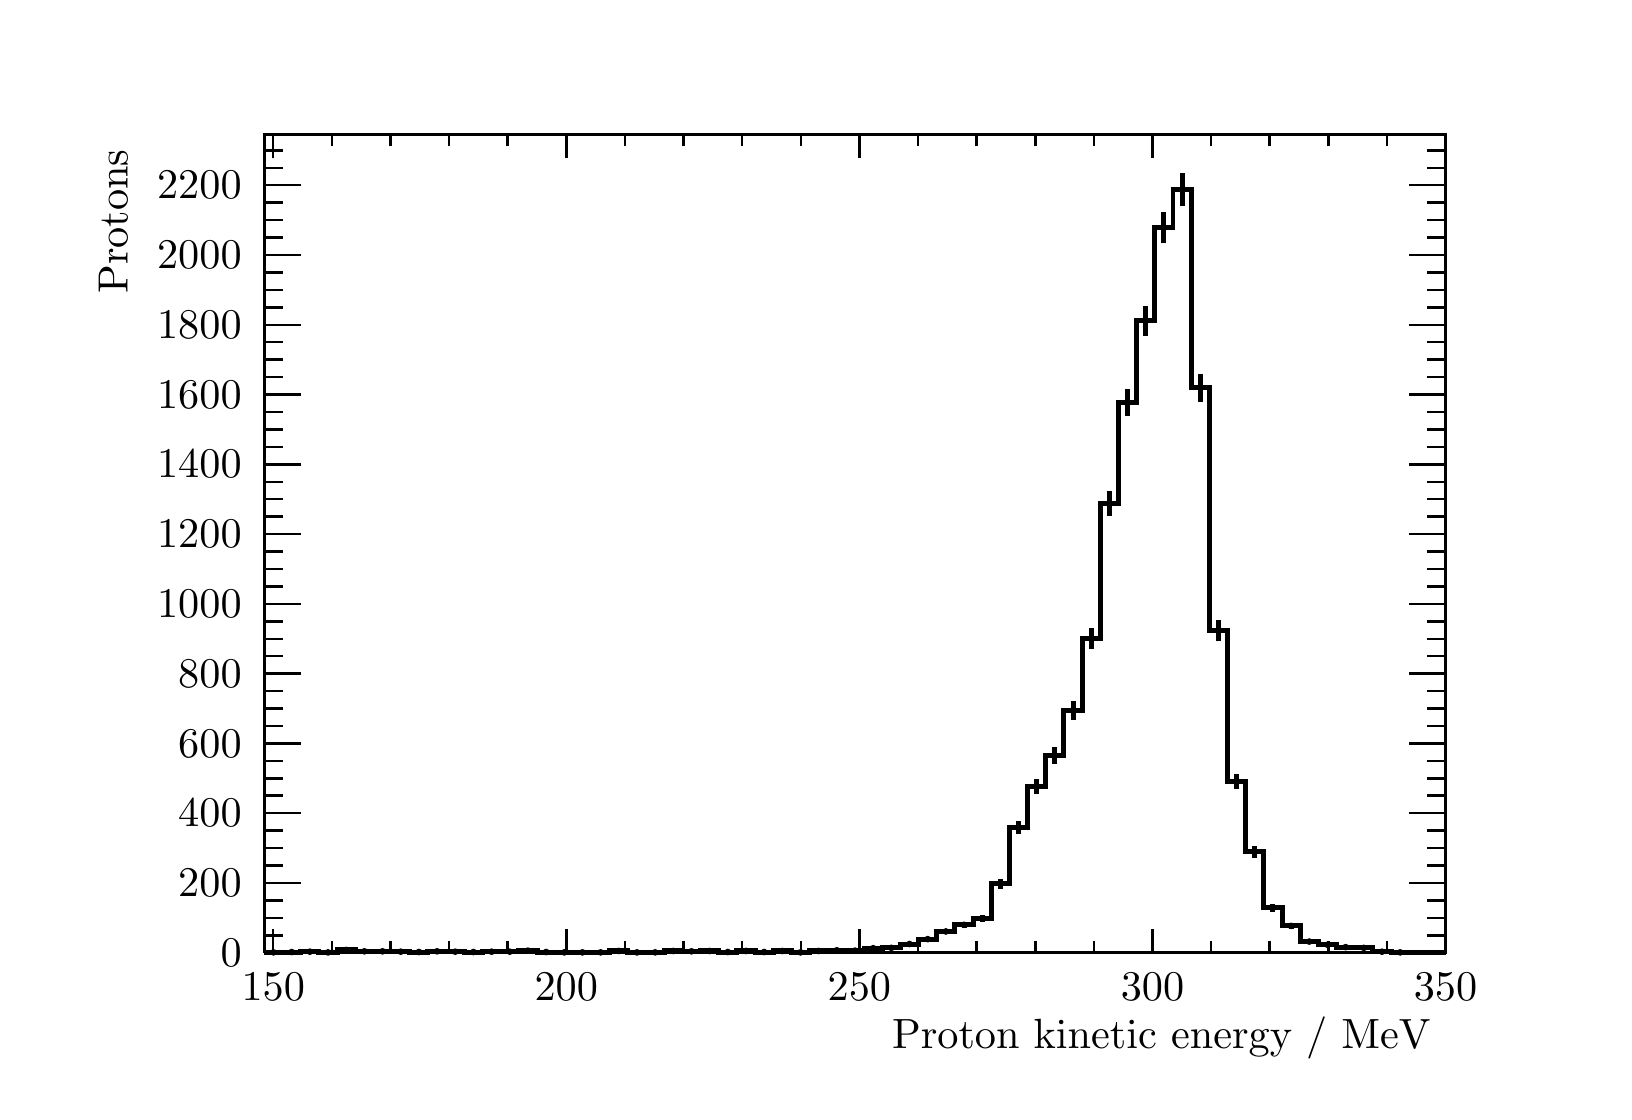
\begin{tikzpicture}
\pgfdeclareplotmark{cross} {
\pgfpathmoveto{\pgfpoint{-0.3\pgfplotmarksize}{\pgfplotmarksize}}
\pgfpathlineto{\pgfpoint{+0.3\pgfplotmarksize}{\pgfplotmarksize}}
\pgfpathlineto{\pgfpoint{+0.3\pgfplotmarksize}{0.3\pgfplotmarksize}}
\pgfpathlineto{\pgfpoint{+1\pgfplotmarksize}{0.3\pgfplotmarksize}}
\pgfpathlineto{\pgfpoint{+1\pgfplotmarksize}{-0.3\pgfplotmarksize}}
\pgfpathlineto{\pgfpoint{+0.3\pgfplotmarksize}{-0.3\pgfplotmarksize}}
\pgfpathlineto{\pgfpoint{+0.3\pgfplotmarksize}{-1.\pgfplotmarksize}}
\pgfpathlineto{\pgfpoint{-0.3\pgfplotmarksize}{-1.\pgfplotmarksize}}
\pgfpathlineto{\pgfpoint{-0.3\pgfplotmarksize}{-0.3\pgfplotmarksize}}
\pgfpathlineto{\pgfpoint{-1.\pgfplotmarksize}{-0.3\pgfplotmarksize}}
\pgfpathlineto{\pgfpoint{-1.\pgfplotmarksize}{0.3\pgfplotmarksize}}
\pgfpathlineto{\pgfpoint{-0.3\pgfplotmarksize}{0.3\pgfplotmarksize}}
\pgfpathclose
\pgfusepathqstroke
}
\pgfdeclareplotmark{cross*} {
\pgfpathmoveto{\pgfpoint{-0.3\pgfplotmarksize}{\pgfplotmarksize}}
\pgfpathlineto{\pgfpoint{+0.3\pgfplotmarksize}{\pgfplotmarksize}}
\pgfpathlineto{\pgfpoint{+0.3\pgfplotmarksize}{0.3\pgfplotmarksize}}
\pgfpathlineto{\pgfpoint{+1\pgfplotmarksize}{0.3\pgfplotmarksize}}
\pgfpathlineto{\pgfpoint{+1\pgfplotmarksize}{-0.3\pgfplotmarksize}}
\pgfpathlineto{\pgfpoint{+0.3\pgfplotmarksize}{-0.3\pgfplotmarksize}}
\pgfpathlineto{\pgfpoint{+0.3\pgfplotmarksize}{-1.\pgfplotmarksize}}
\pgfpathlineto{\pgfpoint{-0.3\pgfplotmarksize}{-1.\pgfplotmarksize}}
\pgfpathlineto{\pgfpoint{-0.3\pgfplotmarksize}{-0.3\pgfplotmarksize}}
\pgfpathlineto{\pgfpoint{-1.\pgfplotmarksize}{-0.3\pgfplotmarksize}}
\pgfpathlineto{\pgfpoint{-1.\pgfplotmarksize}{0.3\pgfplotmarksize}}
\pgfpathlineto{\pgfpoint{-0.3\pgfplotmarksize}{0.3\pgfplotmarksize}}
\pgfpathclose
\pgfusepathqfillstroke
}
\pgfdeclareplotmark{newstar} {
\pgfpathmoveto{\pgfqpoint{0pt}{\pgfplotmarksize}}
\pgfpathlineto{\pgfqpointpolar{44}{0.5\pgfplotmarksize}}
\pgfpathlineto{\pgfqpointpolar{18}{\pgfplotmarksize}}
\pgfpathlineto{\pgfqpointpolar{-20}{0.5\pgfplotmarksize}}
\pgfpathlineto{\pgfqpointpolar{-54}{\pgfplotmarksize}}
\pgfpathlineto{\pgfqpointpolar{-90}{0.5\pgfplotmarksize}}
\pgfpathlineto{\pgfqpointpolar{234}{\pgfplotmarksize}}
\pgfpathlineto{\pgfqpointpolar{198}{0.5\pgfplotmarksize}}
\pgfpathlineto{\pgfqpointpolar{162}{\pgfplotmarksize}}
\pgfpathlineto{\pgfqpointpolar{134}{0.5\pgfplotmarksize}}
\pgfpathclose
\pgfusepathqstroke
}
\pgfdeclareplotmark{newstar*} {
\pgfpathmoveto{\pgfqpoint{0pt}{\pgfplotmarksize}}
\pgfpathlineto{\pgfqpointpolar{44}{0.5\pgfplotmarksize}}
\pgfpathlineto{\pgfqpointpolar{18}{\pgfplotmarksize}}
\pgfpathlineto{\pgfqpointpolar{-20}{0.5\pgfplotmarksize}}
\pgfpathlineto{\pgfqpointpolar{-54}{\pgfplotmarksize}}
\pgfpathlineto{\pgfqpointpolar{-90}{0.5\pgfplotmarksize}}
\pgfpathlineto{\pgfqpointpolar{234}{\pgfplotmarksize}}
\pgfpathlineto{\pgfqpointpolar{198}{0.5\pgfplotmarksize}}
\pgfpathlineto{\pgfqpointpolar{162}{\pgfplotmarksize}}
\pgfpathlineto{\pgfqpointpolar{134}{0.5\pgfplotmarksize}}
\pgfpathclose
\pgfusepathqfillstroke
}
\definecolor{c}{rgb}{1,1,1};
\draw [color=c, fill=c] (0,0) rectangle (20,13.4957);
\draw [color=c, fill=c] (3,1.75444) rectangle (18,12.1461);
\definecolor{c}{rgb}{0,0,0};
\draw [c,line width=0.9] (3,1.75444) -- (3,12.1461) -- (18,12.1461) -- (18,1.75444) -- (3,1.75444);
\definecolor{c}{rgb}{1,1,1};
\draw [color=c, fill=c] (3,1.75444) rectangle (18,12.1461);
\definecolor{c}{rgb}{0,0,0};
\draw [c,line width=0.9] (3,1.75444) -- (3,12.1461) -- (18,12.1461) -- (18,1.75444) -- (3,1.75444);
\draw [c,line width=1.8] (3.11538,1.75444) -- (3.11538,1.75887);
\draw [c,line width=1.8] (3.11538,1.75887) -- (3.11538,1.7633);
\foreach \P in {(3.11538,1.75887)}{\draw[mark options={color=c,fill=c},mark size=2.402402pt,mark=*,mark size=1pt] plot coordinates {\P};}
\draw [c,line width=1.8] (3.34615,1.75704) -- (3.34615,1.7633);
\draw [c,line width=1.8] (3.34615,1.7633) -- (3.34615,1.76957);
\foreach \P in {(3.34615,1.7633)}{\draw[mark options={color=c,fill=c},mark size=2.402402pt,mark=*,mark size=1pt] plot coordinates {\P};}
\draw [c,line width=1.8] (3.57692,1.76006) -- (3.57692,1.76773);
\draw [c,line width=1.8] (3.57692,1.76773) -- (3.57692,1.77541);
\foreach \P in {(3.57692,1.76773)}{\draw[mark options={color=c,fill=c},mark size=2.402402pt,mark=*,mark size=1pt] plot coordinates {\P};}
\draw [c,line width=1.8] (3.80769,1.75444) -- (3.80769,1.75887);
\draw [c,line width=1.8] (3.80769,1.75887) -- (3.80769,1.7633);
\foreach \P in {(3.80769,1.75887)}{\draw[mark options={color=c,fill=c},mark size=2.402402pt,mark=*,mark size=1pt] plot coordinates {\P};}
\draw [c,line width=1.8] (4.03846,1.77735) -- (4.03846,1.78989);
\draw [c,line width=1.8] (4.03846,1.78989) -- (4.03846,1.80242);
\foreach \P in {(4.03846,1.78989)}{\draw[mark options={color=c,fill=c},mark size=2.402402pt,mark=*,mark size=1pt] plot coordinates {\P};}
\draw [c,line width=1.8] (4.26923,1.7633) -- (4.26923,1.77216);
\draw [c,line width=1.8] (4.26923,1.77216) -- (4.26923,1.78102);
\foreach \P in {(4.26923,1.77216)}{\draw[mark options={color=c,fill=c},mark size=2.402402pt,mark=*,mark size=1pt] plot coordinates {\P};}
\draw [c,line width=1.8] (4.5,1.7633) -- (4.5,1.77216);
\draw [c,line width=1.8] (4.5,1.77216) -- (4.5,1.78102);
\foreach \P in {(4.5,1.77216)}{\draw[mark options={color=c,fill=c},mark size=2.402402pt,mark=*,mark size=1pt] plot coordinates {\P};}
\draw [c,line width=1.8] (4.73077,1.76006) -- (4.73077,1.76773);
\draw [c,line width=1.8] (4.73077,1.76773) -- (4.73077,1.77541);
\foreach \P in {(4.73077,1.76773)}{\draw[mark options={color=c,fill=c},mark size=2.402402pt,mark=*,mark size=1pt] plot coordinates {\P};}
\draw [c,line width=1.8] (4.96154,1.75704) -- (4.96154,1.7633);
\draw [c,line width=1.8] (4.96154,1.7633) -- (4.96154,1.76957);
\foreach \P in {(4.96154,1.7633)}{\draw[mark options={color=c,fill=c},mark size=2.402402pt,mark=*,mark size=1pt] plot coordinates {\P};}
\draw [c,line width=1.8] (5.19231,1.7633) -- (5.19231,1.77216);
\draw [c,line width=1.8] (5.19231,1.77216) -- (5.19231,1.78102);
\foreach \P in {(5.19231,1.77216)}{\draw[mark options={color=c,fill=c},mark size=2.402402pt,mark=*,mark size=1pt] plot coordinates {\P};}
\draw [c,line width=1.8] (5.42308,1.76006) -- (5.42308,1.76773);
\draw [c,line width=1.8] (5.42308,1.76773) -- (5.42308,1.77541);
\foreach \P in {(5.42308,1.76773)}{\draw[mark options={color=c,fill=c},mark size=2.402402pt,mark=*,mark size=1pt] plot coordinates {\P};}
\draw [c,line width=1.8] (5.65385,1.75704) -- (5.65385,1.7633);
\draw [c,line width=1.8] (5.65385,1.7633) -- (5.65385,1.76957);
\foreach \P in {(5.65385,1.7633)}{\draw[mark options={color=c,fill=c},mark size=2.402402pt,mark=*,mark size=1pt] plot coordinates {\P};}
\draw [c,line width=1.8] (5.88462,1.76006) -- (5.88462,1.76773);
\draw [c,line width=1.8] (5.88462,1.76773) -- (5.88462,1.77541);
\foreach \P in {(5.88462,1.76773)}{\draw[mark options={color=c,fill=c},mark size=2.402402pt,mark=*,mark size=1pt] plot coordinates {\P};}
\draw [c,line width=1.8] (6.11538,1.76006) -- (6.11538,1.76773);
\draw [c,line width=1.8] (6.11538,1.76773) -- (6.11538,1.77541);
\foreach \P in {(6.11538,1.76773)}{\draw[mark options={color=c,fill=c},mark size=2.402402pt,mark=*,mark size=1pt] plot coordinates {\P};}
\draw [c,line width=1.8] (6.34615,1.77017) -- (6.34615,1.78102);
\draw [c,line width=1.8] (6.34615,1.78102) -- (6.34615,1.79188);
\foreach \P in {(6.34615,1.78102)}{\draw[mark options={color=c,fill=c},mark size=2.402402pt,mark=*,mark size=1pt] plot coordinates {\P};}
\draw [c,line width=1.8] (6.57692,1.75704) -- (6.57692,1.7633);
\draw [c,line width=1.8] (6.57692,1.7633) -- (6.57692,1.76957);
\foreach \P in {(6.57692,1.7633)}{\draw[mark options={color=c,fill=c},mark size=2.402402pt,mark=*,mark size=1pt] plot coordinates {\P};}
\draw [c,line width=1.8] (6.80769,1.75444) -- (6.80769,1.75887);
\draw [c,line width=1.8] (6.80769,1.75887) -- (6.80769,1.7633);
\foreach \P in {(6.80769,1.75887)}{\draw[mark options={color=c,fill=c},mark size=2.402402pt,mark=*,mark size=1pt] plot coordinates {\P};}
\draw [c,line width=1.8] (7.03846,1.75444) -- (7.03846,1.75887);
\draw [c,line width=1.8] (7.03846,1.75887) -- (7.03846,1.7633);
\foreach \P in {(7.03846,1.75887)}{\draw[mark options={color=c,fill=c},mark size=2.402402pt,mark=*,mark size=1pt] plot coordinates {\P};}
\draw [c,line width=1.8] (7.26923,1.75444) -- (7.26923,1.75887);
\draw [c,line width=1.8] (7.26923,1.75887) -- (7.26923,1.7633);
\foreach \P in {(7.26923,1.75887)}{\draw[mark options={color=c,fill=c},mark size=2.402402pt,mark=*,mark size=1pt] plot coordinates {\P};}
\draw [c,line width=1.8] (7.5,1.76669) -- (7.5,1.77659);
\draw [c,line width=1.8] (7.5,1.77659) -- (7.5,1.7865);
\foreach \P in {(7.5,1.77659)}{\draw[mark options={color=c,fill=c},mark size=2.402402pt,mark=*,mark size=1pt] plot coordinates {\P};}
\draw [c,line width=1.8] (7.73077,1.75444) -- (7.73077,1.75887);
\draw [c,line width=1.8] (7.73077,1.75887) -- (7.73077,1.7633);
\foreach \P in {(7.73077,1.75887)}{\draw[mark options={color=c,fill=c},mark size=2.402402pt,mark=*,mark size=1pt] plot coordinates {\P};}
\draw [c,line width=1.8] (7.96154,1.75444) -- (7.96154,1.75887);
\draw [c,line width=1.8] (7.96154,1.75887) -- (7.96154,1.7633);
\foreach \P in {(7.96154,1.75887)}{\draw[mark options={color=c,fill=c},mark size=2.402402pt,mark=*,mark size=1pt] plot coordinates {\P};}
\draw [c,line width=1.8] (8.19231,1.76669) -- (8.19231,1.77659);
\draw [c,line width=1.8] (8.19231,1.77659) -- (8.19231,1.7865);
\foreach \P in {(8.19231,1.77659)}{\draw[mark options={color=c,fill=c},mark size=2.402402pt,mark=*,mark size=1pt] plot coordinates {\P};}
\draw [c,line width=1.8] (8.42308,1.7633) -- (8.42308,1.77216);
\draw [c,line width=1.8] (8.42308,1.77216) -- (8.42308,1.78102);
\foreach \P in {(8.42308,1.77216)}{\draw[mark options={color=c,fill=c},mark size=2.402402pt,mark=*,mark size=1pt] plot coordinates {\P};}
\draw [c,line width=1.8] (8.65385,1.76669) -- (8.65385,1.77659);
\draw [c,line width=1.8] (8.65385,1.77659) -- (8.65385,1.7865);
\foreach \P in {(8.65385,1.77659)}{\draw[mark options={color=c,fill=c},mark size=2.402402pt,mark=*,mark size=1pt] plot coordinates {\P};}
\draw [c,line width=1.8] (8.88462,1.75704) -- (8.88462,1.7633);
\draw [c,line width=1.8] (8.88462,1.7633) -- (8.88462,1.76957);
\foreach \P in {(8.88462,1.7633)}{\draw[mark options={color=c,fill=c},mark size=2.402402pt,mark=*,mark size=1pt] plot coordinates {\P};}
\draw [c,line width=1.8] (9.11539,1.76669) -- (9.11539,1.77659);
\draw [c,line width=1.8] (9.11539,1.77659) -- (9.11539,1.7865);
\foreach \P in {(9.11539,1.77659)}{\draw[mark options={color=c,fill=c},mark size=2.402402pt,mark=*,mark size=1pt] plot coordinates {\P};}
\draw [c,line width=1.8] (9.34615,1.75704) -- (9.34615,1.7633);
\draw [c,line width=1.8] (9.34615,1.7633) -- (9.34615,1.76957);
\foreach \P in {(9.34615,1.7633)}{\draw[mark options={color=c,fill=c},mark size=2.402402pt,mark=*,mark size=1pt] plot coordinates {\P};}
\draw [c,line width=1.8] (9.57692,1.76669) -- (9.57692,1.77659);
\draw [c,line width=1.8] (9.57692,1.77659) -- (9.57692,1.7865);
\foreach \P in {(9.57692,1.77659)}{\draw[mark options={color=c,fill=c},mark size=2.402402pt,mark=*,mark size=1pt] plot coordinates {\P};}
\draw [c,line width=1.8] (9.80769,1.75444) -- (9.80769,1.75887);
\draw [c,line width=1.8] (9.80769,1.75887) -- (9.80769,1.7633);
\foreach \P in {(9.80769,1.75887)}{\draw[mark options={color=c,fill=c},mark size=2.402402pt,mark=*,mark size=1pt] plot coordinates {\P};}
\draw [c,line width=1.8] (10.0385,1.76669) -- (10.0385,1.77659);
\draw [c,line width=1.8] (10.0385,1.77659) -- (10.0385,1.7865);
\foreach \P in {(10.0385,1.77659)}{\draw[mark options={color=c,fill=c},mark size=2.402402pt,mark=*,mark size=1pt] plot coordinates {\P};}
\draw [c,line width=1.8] (10.2692,1.77373) -- (10.2692,1.78546);
\draw [c,line width=1.8] (10.2692,1.78546) -- (10.2692,1.79718);
\foreach \P in {(10.2692,1.78546)}{\draw[mark options={color=c,fill=c},mark size=2.402402pt,mark=*,mark size=1pt] plot coordinates {\P};}
\draw [c,line width=1.8] (10.5,1.77017) -- (10.5,1.78102);
\draw [c,line width=1.8] (10.5,1.78102) -- (10.5,1.79188);
\foreach \P in {(10.5,1.78102)}{\draw[mark options={color=c,fill=c},mark size=2.402402pt,mark=*,mark size=1pt] plot coordinates {\P};}
\draw [c,line width=1.8] (10.7308,1.79606) -- (10.7308,1.81204);
\draw [c,line width=1.8] (10.7308,1.81204) -- (10.7308,1.82801);
\foreach \P in {(10.7308,1.81204)}{\draw[mark options={color=c,fill=c},mark size=2.402402pt,mark=*,mark size=1pt] plot coordinates {\P};}
\draw [c,line width=1.8] (10.9615,1.79989) -- (10.9615,1.81647);
\draw [c,line width=1.8] (10.9615,1.81647) -- (10.9615,1.83305);
\foreach \P in {(10.9615,1.81647)}{\draw[mark options={color=c,fill=c},mark size=2.402402pt,mark=*,mark size=1pt] plot coordinates {\P};}
\draw [c,line width=1.8] (11.1923,1.84305) -- (11.1923,1.86521);
\draw [c,line width=1.8] (11.1923,1.86521) -- (11.1923,1.88736);
\foreach \P in {(11.1923,1.86521)}{\draw[mark options={color=c,fill=c},mark size=2.402402pt,mark=*,mark size=1pt] plot coordinates {\P};}
\draw [c,line width=1.8] (11.4231,1.89956) -- (11.4231,1.92723);
\draw [c,line width=1.8] (11.4231,1.92723) -- (11.4231,1.9549);
\foreach \P in {(11.4231,1.92723)}{\draw[mark options={color=c,fill=c},mark size=2.402402pt,mark=*,mark size=1pt] plot coordinates {\P};}
\draw [c,line width=1.8] (11.6538,1.9901) -- (11.6538,2.02471);
\draw [c,line width=1.8] (11.6538,2.02471) -- (11.6538,2.05931);
\foreach \P in {(11.6538,2.02471)}{\draw[mark options={color=c,fill=c},mark size=2.402402pt,mark=*,mark size=1pt] plot coordinates {\P};}
\draw [c,line width=1.8] (11.8846,2.06926) -- (11.8846,2.10889);
\draw [c,line width=1.8] (11.8846,2.10889) -- (11.8846,2.14851);
\foreach \P in {(11.8846,2.10889)}{\draw[mark options={color=c,fill=c},mark size=2.402402pt,mark=*,mark size=1pt] plot coordinates {\P};}
\draw [c,line width=1.8] (12.1154,2.14478) -- (12.1154,2.18864);
\draw [c,line width=1.8] (12.1154,2.18864) -- (12.1154,2.2325);
\foreach \P in {(12.1154,2.18864)}{\draw[mark options={color=c,fill=c},mark size=2.402402pt,mark=*,mark size=1pt] plot coordinates {\P};}
\draw [c,line width=1.8] (12.3462,2.56935) -- (12.3462,2.63169);
\draw [c,line width=1.8] (12.3462,2.63169) -- (12.3462,2.69404);
\foreach \P in {(12.3462,2.63169)}{\draw[mark options={color=c,fill=c},mark size=2.402402pt,mark=*,mark size=1pt] plot coordinates {\P};}
\draw [c,line width=1.8] (12.5769,3.26538) -- (12.5769,3.34945);
\draw [c,line width=1.8] (12.5769,3.34945) -- (12.5769,3.43351);
\foreach \P in {(12.5769,3.34945)}{\draw[mark options={color=c,fill=c},mark size=2.402402pt,mark=*,mark size=1pt] plot coordinates {\P};}
\draw [c,line width=1.8] (12.8077,3.77106) -- (12.8077,3.86782);
\draw [c,line width=1.8] (12.8077,3.86782) -- (12.8077,3.96459);
\foreach \P in {(12.8077,3.86782)}{\draw[mark options={color=c,fill=c},mark size=2.402402pt,mark=*,mark size=1pt] plot coordinates {\P};}
\draw [c,line width=1.8] (13.0385,4.1524) -- (13.0385,4.25771);
\draw [c,line width=1.8] (13.0385,4.25771) -- (13.0385,4.36303);
\foreach \P in {(13.0385,4.25771)}{\draw[mark options={color=c,fill=c},mark size=2.402402pt,mark=*,mark size=1pt] plot coordinates {\P};}
\draw [c,line width=1.8] (13.2692,4.71254) -- (13.2692,4.82926);
\draw [c,line width=1.8] (13.2692,4.82926) -- (13.2692,4.94597);
\foreach \P in {(13.2692,4.82926)}{\draw[mark options={color=c,fill=c},mark size=2.402402pt,mark=*,mark size=1pt] plot coordinates {\P};}
\draw [c,line width=1.8] (13.5,5.60904) -- (13.5,5.74195);
\draw [c,line width=1.8] (13.5,5.74195) -- (13.5,5.87487);
\foreach \P in {(13.5,5.74195)}{\draw[mark options={color=c,fill=c},mark size=2.402402pt,mark=*,mark size=1pt] plot coordinates {\P};}
\draw [c,line width=1.8] (13.7308,7.302) -- (13.7308,7.46101);
\draw [c,line width=1.8] (13.7308,7.46101) -- (13.7308,7.62002);
\foreach \P in {(13.7308,7.46101)}{\draw[mark options={color=c,fill=c},mark size=2.402402pt,mark=*,mark size=1pt] plot coordinates {\P};}
\draw [c,line width=1.8] (13.9615,8.5655) -- (13.9615,8.74145);
\draw [c,line width=1.8] (13.9615,8.74145) -- (13.9615,8.91739);
\foreach \P in {(13.9615,8.74145)}{\draw[mark options={color=c,fill=c},mark size=2.402402pt,mark=*,mark size=1pt] plot coordinates {\P};}
\draw [c,line width=1.8] (14.1923,9.58965) -- (14.1923,9.7782);
\draw [c,line width=1.8] (14.1923,9.7782) -- (14.1923,9.96675);
\foreach \P in {(14.1923,9.7782)}{\draw[mark options={color=c,fill=c},mark size=2.402402pt,mark=*,mark size=1pt] plot coordinates {\P};}
\draw [c,line width=1.8] (14.4231,10.7636) -- (14.4231,10.9656);
\draw [c,line width=1.8] (14.4231,10.9656) -- (14.4231,11.1676);
\foreach \P in {(14.4231,10.9656)}{\draw[mark options={color=c,fill=c},mark size=2.402402pt,mark=*,mark size=1pt] plot coordinates {\P};}
\draw [c,line width=1.8] (14.6538,11.2369) -- (14.6538,11.4441);
\draw [c,line width=1.8] (14.6538,11.4441) -- (14.6538,11.6513);
\foreach \P in {(14.6538,11.4441)}{\draw[mark options={color=c,fill=c},mark size=2.402402pt,mark=*,mark size=1pt] plot coordinates {\P};}
\draw [c,line width=1.8] (14.8846,8.75363) -- (14.8846,8.93196);
\draw [c,line width=1.8] (14.8846,8.93196) -- (14.8846,9.11029);
\foreach \P in {(14.8846,8.93196)}{\draw[mark options={color=c,fill=c},mark size=2.402402pt,mark=*,mark size=1pt] plot coordinates {\P};}
\draw [c,line width=1.8] (15.1154,5.70925) -- (15.1154,5.84385);
\draw [c,line width=1.8] (15.1154,5.84385) -- (15.1154,5.97846);
\foreach \P in {(15.1154,5.84385)}{\draw[mark options={color=c,fill=c},mark size=2.402402pt,mark=*,mark size=1pt] plot coordinates {\P};}
\draw [c,line width=1.8] (15.3462,3.83168) -- (15.3462,3.92985);
\draw [c,line width=1.8] (15.3462,3.92985) -- (15.3462,4.02802);
\foreach \P in {(15.3462,3.92985)}{\draw[mark options={color=c,fill=c},mark size=2.402402pt,mark=*,mark size=1pt] plot coordinates {\P};}
\draw [c,line width=1.8] (15.5769,2.95956) -- (15.5769,3.03488);
\draw [c,line width=1.8] (15.5769,3.03488) -- (15.5769,3.11019);
\foreach \P in {(15.5769,3.03488)}{\draw[mark options={color=c,fill=c},mark size=2.402402pt,mark=*,mark size=1pt] plot coordinates {\P};}
\draw [c,line width=1.8] (15.8077,2.27566) -- (15.8077,2.32598);
\draw [c,line width=1.8] (15.8077,2.32598) -- (15.8077,2.37631);
\foreach \P in {(15.8077,2.32598)}{\draw[mark options={color=c,fill=c},mark size=2.402402pt,mark=*,mark size=1pt] plot coordinates {\P};}
\draw [c,line width=1.8] (16.0385,2.05672) -- (16.0385,2.09559);
\draw [c,line width=1.8] (16.0385,2.09559) -- (16.0385,2.13447);
\foreach \P in {(16.0385,2.09559)}{\draw[mark options={color=c,fill=c},mark size=2.402402pt,mark=*,mark size=1pt] plot coordinates {\P};}
\draw [c,line width=1.8] (16.2692,1.87116) -- (16.2692,1.89622);
\draw [c,line width=1.8] (16.2692,1.89622) -- (16.2692,1.92128);
\foreach \P in {(16.2692,1.89622)}{\draw[mark options={color=c,fill=c},mark size=2.402402pt,mark=*,mark size=1pt] plot coordinates {\P};}
\draw [c,line width=1.8] (16.5,1.8351) -- (16.5,1.85634);
\draw [c,line width=1.8] (16.5,1.85634) -- (16.5,1.87759);
\foreach \P in {(16.5,1.85634)}{\draw[mark options={color=c,fill=c},mark size=2.402402pt,mark=*,mark size=1pt] plot coordinates {\P};}
\draw [c,line width=1.8] (16.7308,1.80761) -- (16.7308,1.82533);
\draw [c,line width=1.8] (16.7308,1.82533) -- (16.7308,1.84305);
\foreach \P in {(16.7308,1.82533)}{\draw[mark options={color=c,fill=c},mark size=2.402402pt,mark=*,mark size=1pt] plot coordinates {\P};}
\draw [c,line width=1.8] (16.9615,1.79989) -- (16.9615,1.81647);
\draw [c,line width=1.8] (16.9615,1.81647) -- (16.9615,1.83305);
\foreach \P in {(16.9615,1.81647)}{\draw[mark options={color=c,fill=c},mark size=2.402402pt,mark=*,mark size=1pt] plot coordinates {\P};}
\draw [c,line width=1.8] (17.1923,1.76006) -- (17.1923,1.76773);
\draw [c,line width=1.8] (17.1923,1.76773) -- (17.1923,1.77541);
\foreach \P in {(17.1923,1.76773)}{\draw[mark options={color=c,fill=c},mark size=2.402402pt,mark=*,mark size=1pt] plot coordinates {\P};}
\draw [c,line width=1.8] (17.4231,1.75444) -- (17.4231,1.75887);
\draw [c,line width=1.8] (17.4231,1.75887) -- (17.4231,1.7633);
\foreach \P in {(17.4231,1.75887)}{\draw[mark options={color=c,fill=c},mark size=2.402402pt,mark=*,mark size=1pt] plot coordinates {\P};}
\draw [c,line width=1.8] (3,1.75887) -- (3.23077,1.75887) -- (3.23077,1.7633) -- (3.46154,1.7633) -- (3.46154,1.76773) -- (3.69231,1.76773) -- (3.69231,1.75887) -- (3.92308,1.75887) -- (3.92308,1.78989) -- (4.15385,1.78989) -- (4.15385,1.77216) --
 (4.38462,1.77216) -- (4.38462,1.77216) -- (4.61538,1.77216) -- (4.61538,1.76773) -- (4.84615,1.76773) -- (4.84615,1.7633) -- (5.07692,1.7633) -- (5.07692,1.77216) -- (5.30769,1.77216) -- (5.30769,1.76773) -- (5.53846,1.76773) -- (5.53846,1.7633) --
 (5.76923,1.7633) -- (5.76923,1.76773) -- (6,1.76773) -- (6,1.76773) -- (6.23077,1.76773) -- (6.23077,1.78102) -- (6.46154,1.78102) -- (6.46154,1.7633) -- (6.69231,1.7633) -- (6.69231,1.75887) -- (6.92308,1.75887) -- (6.92308,1.75887) --
 (7.15385,1.75887) -- (7.15385,1.75887) -- (7.38462,1.75887) -- (7.38462,1.77659) -- (7.61538,1.77659) -- (7.61538,1.75887) -- (7.84615,1.75887) -- (7.84615,1.75887) -- (8.07692,1.75887) -- (8.07692,1.77659) -- (8.30769,1.77659) -- (8.30769,1.77216)
 -- (8.53846,1.77216) -- (8.53846,1.77659) -- (8.76923,1.77659) -- (8.76923,1.7633) -- (9,1.7633) -- (9,1.77659) -- (9.23077,1.77659) -- (9.23077,1.7633) -- (9.46154,1.7633) -- (9.46154,1.77659) -- (9.69231,1.77659) -- (9.69231,1.75887) --
 (9.92308,1.75887) -- (9.92308,1.77659) -- (10.1538,1.77659) -- (10.1538,1.78546) -- (10.3846,1.78546) -- (10.3846,1.78102) -- (10.6154,1.78102) -- (10.6154,1.81204) -- (10.8462,1.81204) -- (10.8462,1.81647) -- (11.0769,1.81647) -- (11.0769,1.86521)
 -- (11.3077,1.86521) -- (11.3077,1.92723) -- (11.5385,1.92723) -- (11.5385,2.02471) -- (11.7692,2.02471) -- (11.7692,2.10889) -- (12,2.10889) -- (12,2.18864) -- (12.2308,2.18864) -- (12.2308,2.63169) -- (12.4615,2.63169) -- (12.4615,3.34945) --
 (12.6923,3.34945) -- (12.6923,3.86782) -- (12.9231,3.86782) -- (12.9231,4.25771) -- (13.1538,4.25771) -- (13.1538,4.82926) -- (13.3846,4.82926) -- (13.3846,5.74195) -- (13.6154,5.74195) -- (13.6154,7.46101) -- (13.8462,7.46101) -- (13.8462,8.74145)
 -- (14.0769,8.74145) -- (14.0769,9.7782) -- (14.3077,9.7782) -- (14.3077,10.9656) -- (14.5385,10.9656) -- (14.5385,11.4441) -- (14.7692,11.4441) -- (14.7692,8.93196) -- (15,8.93196) -- (15,5.84385) -- (15.2308,5.84385) -- (15.2308,3.92985) --
 (15.4615,3.92985) -- (15.4615,3.03488) -- (15.6923,3.03488) -- (15.6923,2.32598) -- (15.9231,2.32598) -- (15.9231,2.09559) -- (16.1538,2.09559) -- (16.1538,1.89622) -- (16.3846,1.89622) -- (16.3846,1.85634) -- (16.6154,1.85634) -- (16.6154,1.82533)
 -- (16.8462,1.82533) -- (16.8462,1.81647) -- (17.0769,1.81647) -- (17.0769,1.76773) -- (17.3077,1.76773) -- (17.3077,1.75887) -- (17.5385,1.75887) -- (17.5385,1.75444) -- (17.7692,1.75444) -- (17.7692,1.75444) -- (18,1.75444);
\draw [c,line width=0.9] (3,1.75444) -- (18,1.75444);
\draw [c,line width=0.9] (3.11166,2.05809) -- (3.11166,1.75444);
\draw [c,line width=0.9] (3.85608,1.90627) -- (3.85608,1.75444);
\draw [c,line width=0.9] (4.6005,1.90627) -- (4.6005,1.75444);
\draw [c,line width=0.9] (5.34491,1.90627) -- (5.34491,1.75444);
\draw [c,line width=0.9] (6.08933,1.90627) -- (6.08933,1.75444);
\draw [c,line width=0.9] (6.83375,2.05809) -- (6.83375,1.75444);
\draw [c,line width=0.9] (7.57816,1.90627) -- (7.57816,1.75444);
\draw [c,line width=0.9] (8.32258,1.90627) -- (8.32258,1.75444);
\draw [c,line width=0.9] (9.067,1.90627) -- (9.067,1.75444);
\draw [c,line width=0.9] (9.81141,1.90627) -- (9.81141,1.75444);
\draw [c,line width=0.9] (10.5558,2.05809) -- (10.5558,1.75444);
\draw [c,line width=0.9] (11.3002,1.90627) -- (11.3002,1.75444);
\draw [c,line width=0.9] (12.0447,1.90627) -- (12.0447,1.75444);
\draw [c,line width=0.9] (12.7891,1.90627) -- (12.7891,1.75444);
\draw [c,line width=0.9] (13.5335,1.90627) -- (13.5335,1.75444);
\draw [c,line width=0.9] (14.2779,2.05809) -- (14.2779,1.75444);
\draw [c,line width=0.9] (15.0223,1.90627) -- (15.0223,1.75444);
\draw [c,line width=0.9] (15.7667,1.90627) -- (15.7667,1.75444);
\draw [c,line width=0.9] (16.5112,1.90627) -- (16.5112,1.75444);
\draw [c,line width=0.9] (17.2556,1.90627) -- (17.2556,1.75444);
\draw [c,line width=0.9] (18,2.05809) -- (18,1.75444);
\draw [c,line width=0.9] (3.11166,2.05809) -- (3.11166,1.75444);
\draw [c,line width=0.9] (18,2.05809) -- (18,1.75444);
\draw [anchor=base] (3.11166,1.14713) node[scale=1.52731, color=c, rotate=0]{150};
\draw [anchor=base] (6.83375,1.14713) node[scale=1.52731, color=c, rotate=0]{200};
\draw [anchor=base] (10.5558,1.14713) node[scale=1.52731, color=c, rotate=0]{250};
\draw [anchor=base] (14.2779,1.14713) node[scale=1.52731, color=c, rotate=0]{300};
\draw [anchor=base] (18,1.14713) node[scale=1.52731, color=c, rotate=0]{350};
\draw [anchor= east] (18,0.674785) node[scale=1.52731, color=c, rotate=0]{ Proton kinetic energy / MeV};
\draw [c,line width=0.9] (3,12.1461) -- (18,12.1461);
\draw [c,line width=0.9] (3.11166,11.8425) -- (3.11166,12.1461);
\draw [c,line width=0.9] (3.85608,11.9943) -- (3.85608,12.1461);
\draw [c,line width=0.9] (4.6005,11.9943) -- (4.6005,12.1461);
\draw [c,line width=0.9] (5.34491,11.9943) -- (5.34491,12.1461);
\draw [c,line width=0.9] (6.08933,11.9943) -- (6.08933,12.1461);
\draw [c,line width=0.9] (6.83375,11.8425) -- (6.83375,12.1461);
\draw [c,line width=0.9] (7.57816,11.9943) -- (7.57816,12.1461);
\draw [c,line width=0.9] (8.32258,11.9943) -- (8.32258,12.1461);
\draw [c,line width=0.9] (9.067,11.9943) -- (9.067,12.1461);
\draw [c,line width=0.9] (9.81141,11.9943) -- (9.81141,12.1461);
\draw [c,line width=0.9] (10.5558,11.8425) -- (10.5558,12.1461);
\draw [c,line width=0.9] (11.3002,11.9943) -- (11.3002,12.1461);
\draw [c,line width=0.9] (12.0447,11.9943) -- (12.0447,12.1461);
\draw [c,line width=0.9] (12.7891,11.9943) -- (12.7891,12.1461);
\draw [c,line width=0.9] (13.5335,11.9943) -- (13.5335,12.1461);
\draw [c,line width=0.9] (14.2779,11.8425) -- (14.2779,12.1461);
\draw [c,line width=0.9] (15.0223,11.9943) -- (15.0223,12.1461);
\draw [c,line width=0.9] (15.7667,11.9943) -- (15.7667,12.1461);
\draw [c,line width=0.9] (16.5112,11.9943) -- (16.5112,12.1461);
\draw [c,line width=0.9] (17.2556,11.9943) -- (17.2556,12.1461);
\draw [c,line width=0.9] (18,11.8425) -- (18,12.1461);
\draw [c,line width=0.9] (3.11166,11.8425) -- (3.11166,12.1461);
\draw [c,line width=0.9] (18,11.8425) -- (18,12.1461);
\draw [c,line width=0.9] (3,1.75444) -- (3,12.1461);
\draw [c,line width=0.9] (3.462,1.75444) -- (3,1.75444);
\draw [c,line width=0.9] (3.231,1.97597) -- (3,1.97597);
\draw [c,line width=0.9] (3.231,2.1975) -- (3,2.1975);
\draw [c,line width=0.9] (3.231,2.41903) -- (3,2.41903);
\draw [c,line width=0.9] (3.462,2.64055) -- (3,2.64055);
\draw [c,line width=0.9] (3.231,2.86208) -- (3,2.86208);
\draw [c,line width=0.9] (3.231,3.08361) -- (3,3.08361);
\draw [c,line width=0.9] (3.231,3.30514) -- (3,3.30514);
\draw [c,line width=0.9] (3.462,3.52667) -- (3,3.52667);
\draw [c,line width=0.9] (3.231,3.7482) -- (3,3.7482);
\draw [c,line width=0.9] (3.231,3.96972) -- (3,3.96972);
\draw [c,line width=0.9] (3.231,4.19125) -- (3,4.19125);
\draw [c,line width=0.9] (3.462,4.41278) -- (3,4.41278);
\draw [c,line width=0.9] (3.231,4.63431) -- (3,4.63431);
\draw [c,line width=0.9] (3.231,4.85584) -- (3,4.85584);
\draw [c,line width=0.9] (3.231,5.07737) -- (3,5.07737);
\draw [c,line width=0.9] (3.462,5.29889) -- (3,5.29889);
\draw [c,line width=0.9] (3.231,5.52042) -- (3,5.52042);
\draw [c,line width=0.9] (3.231,5.74195) -- (3,5.74195);
\draw [c,line width=0.9] (3.231,5.96348) -- (3,5.96348);
\draw [c,line width=0.9] (3.462,6.18501) -- (3,6.18501);
\draw [c,line width=0.9] (3.231,6.40654) -- (3,6.40654);
\draw [c,line width=0.9] (3.231,6.62807) -- (3,6.62807);
\draw [c,line width=0.9] (3.231,6.84959) -- (3,6.84959);
\draw [c,line width=0.9] (3.462,7.07112) -- (3,7.07112);
\draw [c,line width=0.9] (3.231,7.29265) -- (3,7.29265);
\draw [c,line width=0.9] (3.231,7.51418) -- (3,7.51418);
\draw [c,line width=0.9] (3.231,7.73571) -- (3,7.73571);
\draw [c,line width=0.9] (3.462,7.95724) -- (3,7.95724);
\draw [c,line width=0.9] (3.231,8.17876) -- (3,8.17876);
\draw [c,line width=0.9] (3.231,8.40029) -- (3,8.40029);
\draw [c,line width=0.9] (3.231,8.62182) -- (3,8.62182);
\draw [c,line width=0.9] (3.462,8.84335) -- (3,8.84335);
\draw [c,line width=0.9] (3.231,9.06488) -- (3,9.06488);
\draw [c,line width=0.9] (3.231,9.28641) -- (3,9.28641);
\draw [c,line width=0.9] (3.231,9.50793) -- (3,9.50793);
\draw [c,line width=0.9] (3.462,9.72946) -- (3,9.72946);
\draw [c,line width=0.9] (3.231,9.95099) -- (3,9.95099);
\draw [c,line width=0.9] (3.231,10.1725) -- (3,10.1725);
\draw [c,line width=0.9] (3.231,10.394) -- (3,10.394);
\draw [c,line width=0.9] (3.462,10.6156) -- (3,10.6156);
\draw [c,line width=0.9] (3.231,10.8371) -- (3,10.8371);
\draw [c,line width=0.9] (3.231,11.0586) -- (3,11.0586);
\draw [c,line width=0.9] (3.231,11.2802) -- (3,11.2802);
\draw [c,line width=0.9] (3.462,11.5017) -- (3,11.5017);
\draw [c,line width=0.9] (3.462,11.5017) -- (3,11.5017);
\draw [c,line width=0.9] (3.231,11.7232) -- (3,11.7232);
\draw [c,line width=0.9] (3.231,11.9447) -- (3,11.9447);
\draw [anchor= east] (2.9,1.75444) node[scale=1.52731, color=c, rotate=0]{0};
\draw [anchor= east] (2.9,2.64055) node[scale=1.52731, color=c, rotate=0]{200};
\draw [anchor= east] (2.9,3.52667) node[scale=1.52731, color=c, rotate=0]{400};
\draw [anchor= east] (2.9,4.41278) node[scale=1.52731, color=c, rotate=0]{600};
\draw [anchor= east] (2.9,5.29889) node[scale=1.52731, color=c, rotate=0]{800};
\draw [anchor= east] (2.9,6.18501) node[scale=1.52731, color=c, rotate=0]{1000};
\draw [anchor= east] (2.9,7.07112) node[scale=1.52731, color=c, rotate=0]{1200};
\draw [anchor= east] (2.9,7.95724) node[scale=1.52731, color=c, rotate=0]{1400};
\draw [anchor= east] (2.9,8.84335) node[scale=1.52731, color=c, rotate=0]{1600};
\draw [anchor= east] (2.9,9.72946) node[scale=1.52731, color=c, rotate=0]{1800};
\draw [anchor= east] (2.9,10.6156) node[scale=1.52731, color=c, rotate=0]{2000};
\draw [anchor= east] (2.9,11.5017) node[scale=1.52731, color=c, rotate=0]{2200};
\draw [anchor= east] (1.08,12.1461) node[scale=1.52731, color=c, rotate=90]{Protons};
\draw [c,line width=0.9] (18,1.75444) -- (18,12.1461);
\draw [c,line width=0.9] (17.538,1.75444) -- (18,1.75444);
\draw [c,line width=0.9] (17.769,1.97597) -- (18,1.97597);
\draw [c,line width=0.9] (17.769,2.1975) -- (18,2.1975);
\draw [c,line width=0.9] (17.769,2.41903) -- (18,2.41903);
\draw [c,line width=0.9] (17.538,2.64055) -- (18,2.64055);
\draw [c,line width=0.9] (17.769,2.86208) -- (18,2.86208);
\draw [c,line width=0.9] (17.769,3.08361) -- (18,3.08361);
\draw [c,line width=0.9] (17.769,3.30514) -- (18,3.30514);
\draw [c,line width=0.9] (17.538,3.52667) -- (18,3.52667);
\draw [c,line width=0.9] (17.769,3.7482) -- (18,3.7482);
\draw [c,line width=0.9] (17.769,3.96972) -- (18,3.96972);
\draw [c,line width=0.9] (17.769,4.19125) -- (18,4.19125);
\draw [c,line width=0.9] (17.538,4.41278) -- (18,4.41278);
\draw [c,line width=0.9] (17.769,4.63431) -- (18,4.63431);
\draw [c,line width=0.9] (17.769,4.85584) -- (18,4.85584);
\draw [c,line width=0.9] (17.769,5.07737) -- (18,5.07737);
\draw [c,line width=0.9] (17.538,5.29889) -- (18,5.29889);
\draw [c,line width=0.9] (17.769,5.52042) -- (18,5.52042);
\draw [c,line width=0.9] (17.769,5.74195) -- (18,5.74195);
\draw [c,line width=0.9] (17.769,5.96348) -- (18,5.96348);
\draw [c,line width=0.9] (17.538,6.18501) -- (18,6.18501);
\draw [c,line width=0.9] (17.769,6.40654) -- (18,6.40654);
\draw [c,line width=0.9] (17.769,6.62807) -- (18,6.62807);
\draw [c,line width=0.9] (17.769,6.84959) -- (18,6.84959);
\draw [c,line width=0.9] (17.538,7.07112) -- (18,7.07112);
\draw [c,line width=0.9] (17.769,7.29265) -- (18,7.29265);
\draw [c,line width=0.9] (17.769,7.51418) -- (18,7.51418);
\draw [c,line width=0.9] (17.769,7.73571) -- (18,7.73571);
\draw [c,line width=0.9] (17.538,7.95724) -- (18,7.95724);
\draw [c,line width=0.9] (17.769,8.17876) -- (18,8.17876);
\draw [c,line width=0.9] (17.769,8.40029) -- (18,8.40029);
\draw [c,line width=0.9] (17.769,8.62182) -- (18,8.62182);
\draw [c,line width=0.9] (17.538,8.84335) -- (18,8.84335);
\draw [c,line width=0.9] (17.769,9.06488) -- (18,9.06488);
\draw [c,line width=0.9] (17.769,9.28641) -- (18,9.28641);
\draw [c,line width=0.9] (17.769,9.50793) -- (18,9.50793);
\draw [c,line width=0.9] (17.538,9.72946) -- (18,9.72946);
\draw [c,line width=0.9] (17.769,9.95099) -- (18,9.95099);
\draw [c,line width=0.9] (17.769,10.1725) -- (18,10.1725);
\draw [c,line width=0.9] (17.769,10.394) -- (18,10.394);
\draw [c,line width=0.9] (17.538,10.6156) -- (18,10.6156);
\draw [c,line width=0.9] (17.769,10.8371) -- (18,10.8371);
\draw [c,line width=0.9] (17.769,11.0586) -- (18,11.0586);
\draw [c,line width=0.9] (17.769,11.2802) -- (18,11.2802);
\draw [c,line width=0.9] (17.538,11.5017) -- (18,11.5017);
\draw [c,line width=0.9] (17.538,11.5017) -- (18,11.5017);
\draw [c,line width=0.9] (17.769,11.7232) -- (18,11.7232);
\draw [c,line width=0.9] (17.769,11.9447) -- (18,11.9447);
\definecolor{c}{rgb}{1,1,1};
\draw [color=c, fill=c] (2,12.686) rectangle (18,13.4282);
\definecolor{c}{rgb}{0,0,0};
%\draw (10,13.0571) node[scale=1.40004, color=c, rotate=0]{Proton kinetic energy measured in $\mathit{S3}$};
\end{tikzpicture}

    \end{adjustbox}
  \end{minipage}
  \caption{\label{fig:utofNoBend}Measurements of the unmoderated and unbent T10 beam over a baseline of 10.8~m for a selected beam momentum of 0.8~GeV/c. Measurements are made in the $\mathit{S3}$ detector. The peak between 50~ns and 60~ns is produced by protons. Left: Time of flight spectrum. Right: Measured kinetic energy of protons.}
\end{figure}

To enhance the low energy proton flux, a novel technique was employed:
we placed acrylic moderator blocks directly in the beamline, which spread and slowed the beam particles via multiple Coulomb scattering.
By placing the TPC in an off-axis position with respect to the beam direction, we observed a beam composition with lower-energy protons than would otherwise have been possible in the T10 beamline.
These techniques were designed to increase the ratio of protons to MIPs in the TPC, and to decrease the proton momentum and multiplicity in the active region of the TPC.

The flux and composition of beam particles were measured with two ToF systems, placed upstream and downstream of the TPC.
Measurements of protons and MIPs are presented as a function of the off-axis angle and thickness of the moderator.
This paper provides a detailed description of the time of flight systems employed in the beamline in Section~\ref{hptpcPaper:sec:Methods}, the analysis methodology of the ToF data in Section~\ref{hptpcPaper:sec:Analysis}, presentation of the ToF system results in Section~\ref{hptpcPaper:sec:Results}, and additional conclusions in Section~\ref{hptpcPaper:sec:Conclusion}.
